\documentclass[11pt]{article}
\usepackage[textwidth=18.0cm, textheight=23.0cm, top=2.0cm]{geometry}
\usepackage{pst-all}
\usepackage{amssymb}
\usepackage{tikz}
\usepackage{underscore}\begin{document}
\pagestyle{empty}


ClassName: \underline{\textbf{Class_07.2bp-36}}
\par
BinSize: \underline{\textbf{100 × 100}}
\par
ReduceSize: \underline{\textbf{100 × 100}}
\par
TypeNum: \underline{\textbf{80}}
\par
Num: \underline{\textbf{80}}
\par
OutS: \underline{\textbf{240000}}
\par
InS: \underline{\textbf{206353}}
\par
Rate: \underline{\textbf{0.860}}
\par
UB: \underline{\textbf{24}}
\par
LB0: \underline{\textbf{24}}
\par
LB: \underline{\textbf{24}}
\par
LBWithCut: \underline{\textbf{24}}
\par
NodeCut: \underline{\textbf{0}}
\par
ExtendedNodeCnt: \underline{\textbf{1}}
\par
GenNodeCnt: \underline{\textbf{1}}
\par
PrimalNode: \underline{\textbf{0}}
\par
ColumnCount: \underline{\textbf{24}}
\par
TotalCutCount: \underline{\textbf{0}}
\par
RootCutCount: \underline{\textbf{0}}
\par
LPSolverCnt: \underline{\textbf{1}}
\par
PricingSolverCnt: \underline{\textbf{0}}
\par
BranchAndBoundNum: \underline{\textbf{1}}
\par
isOpt: \underline{\textbf{true}}
\par
TimeOnInitSolution: \underline{\textbf{600.000 s}}
\par
TimeOnPrimal: \underline{\textbf{0.000 s}}
\par
TimeOnPricing: \underline{\textbf{0.000 s}}
\par
TimeOnRmp: \underline{\textbf{0.079 s}}
\par
TotalTime: \underline{\textbf{600.352 s}}
\par
\newpage


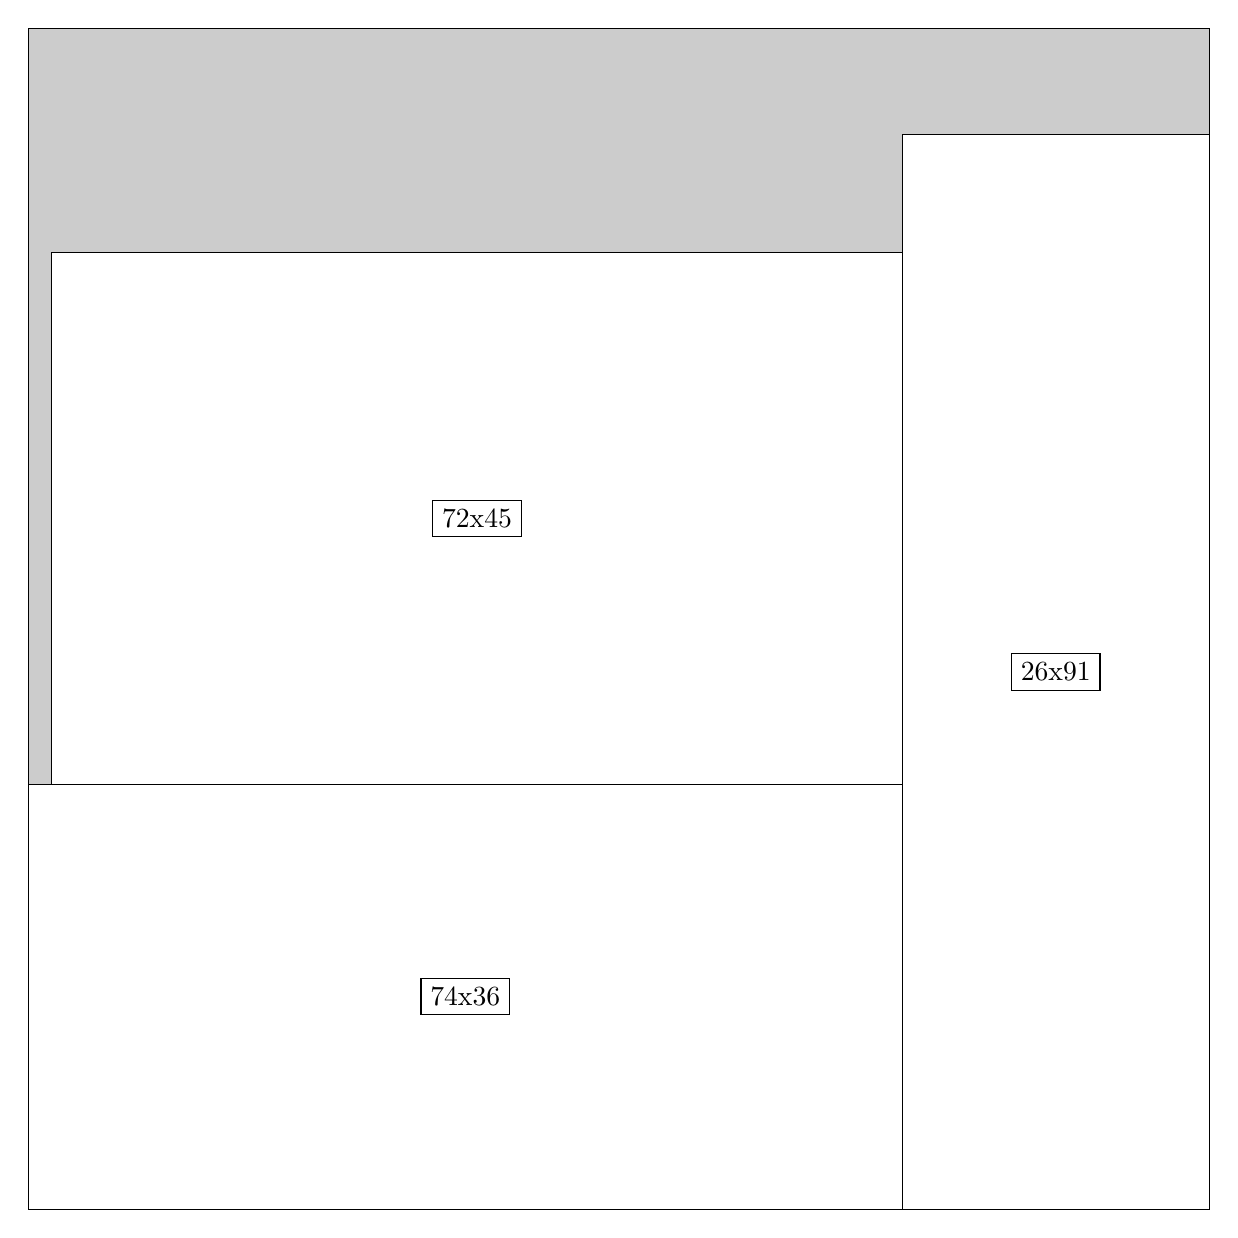
\begin{tikzpicture}[shorten >=1pt,scale=1.0,every node/.style={scale=1.0},->]
\tikzstyle{vertex}=[circle,fill=black!25,minimum size=14pt,inner sep=0pt]
\filldraw[fill=gray!40!white, draw=black] (0,0) rectangle (15.0,15.0);
\foreach \name/\x/\y/\w/\h in {26x91/11.1/0.0/3.9/13.65,74x36/0.0/0.0/11.1/5.3999999999999995,72x45/0.3/5.3999999999999995/10.799999999999999/6.75}
\filldraw[fill=white!40!white, draw=black] (\x,\y) rectangle node[draw] (\name) {\name} ++(\w,\h);
\end{tikzpicture}


w =26 , h =91 , x =74 , y =0 , v =2366
\par
w =74 , h =36 , x =0 , y =0 , v =2664
\par
w =72 , h =45 , x =2 , y =36 , v =3240
\par
\newpage


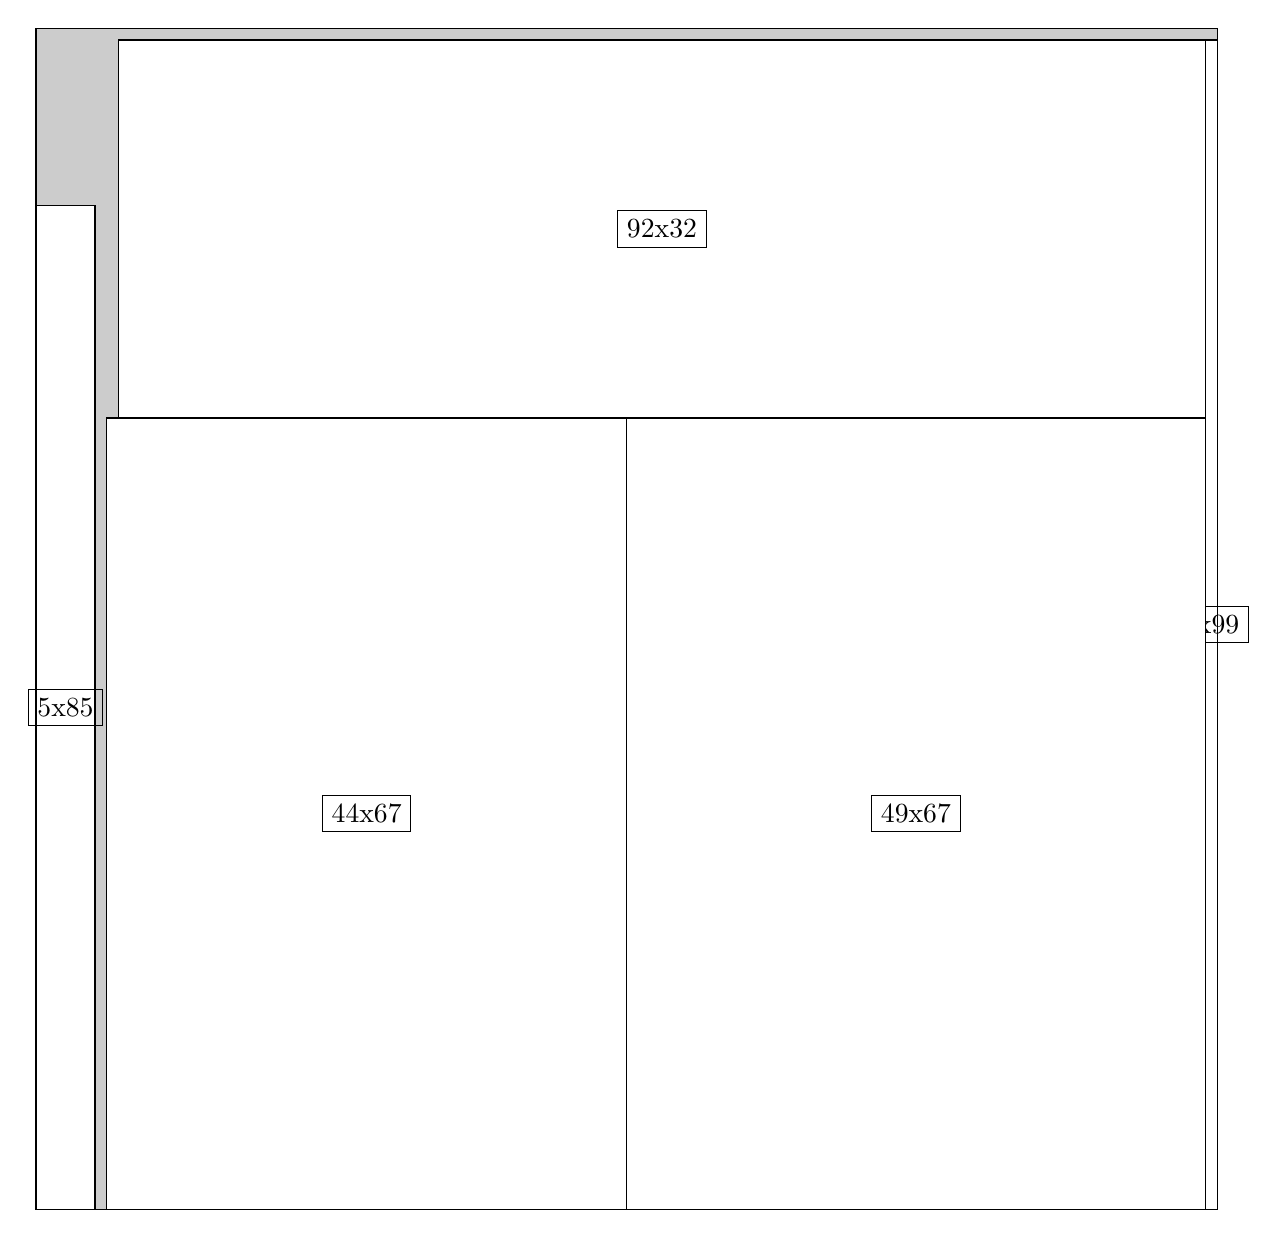
\begin{tikzpicture}[shorten >=1pt,scale=1.0,every node/.style={scale=1.0},->]
\tikzstyle{vertex}=[circle,fill=black!25,minimum size=14pt,inner sep=0pt]
\filldraw[fill=gray!40!white, draw=black] (0,0) rectangle (15.0,15.0);
\foreach \name/\x/\y/\w/\h in {1x99/14.85/0.0/0.15/14.85,49x67/7.5/0.0/7.35/10.049999999999999,44x67/0.8999999999999999/0.0/6.6/10.049999999999999,92x32/1.05/10.049999999999999/13.799999999999999/4.8,5x85/0.0/0.0/0.75/12.75}
\filldraw[fill=white!40!white, draw=black] (\x,\y) rectangle node[draw] (\name) {\name} ++(\w,\h);
\end{tikzpicture}


w =1 , h =99 , x =99 , y =0 , v =99
\par
w =49 , h =67 , x =50 , y =0 , v =3283
\par
w =44 , h =67 , x =6 , y =0 , v =2948
\par
w =92 , h =32 , x =7 , y =67 , v =2944
\par
w =5 , h =85 , x =0 , y =0 , v =425
\par
\newpage


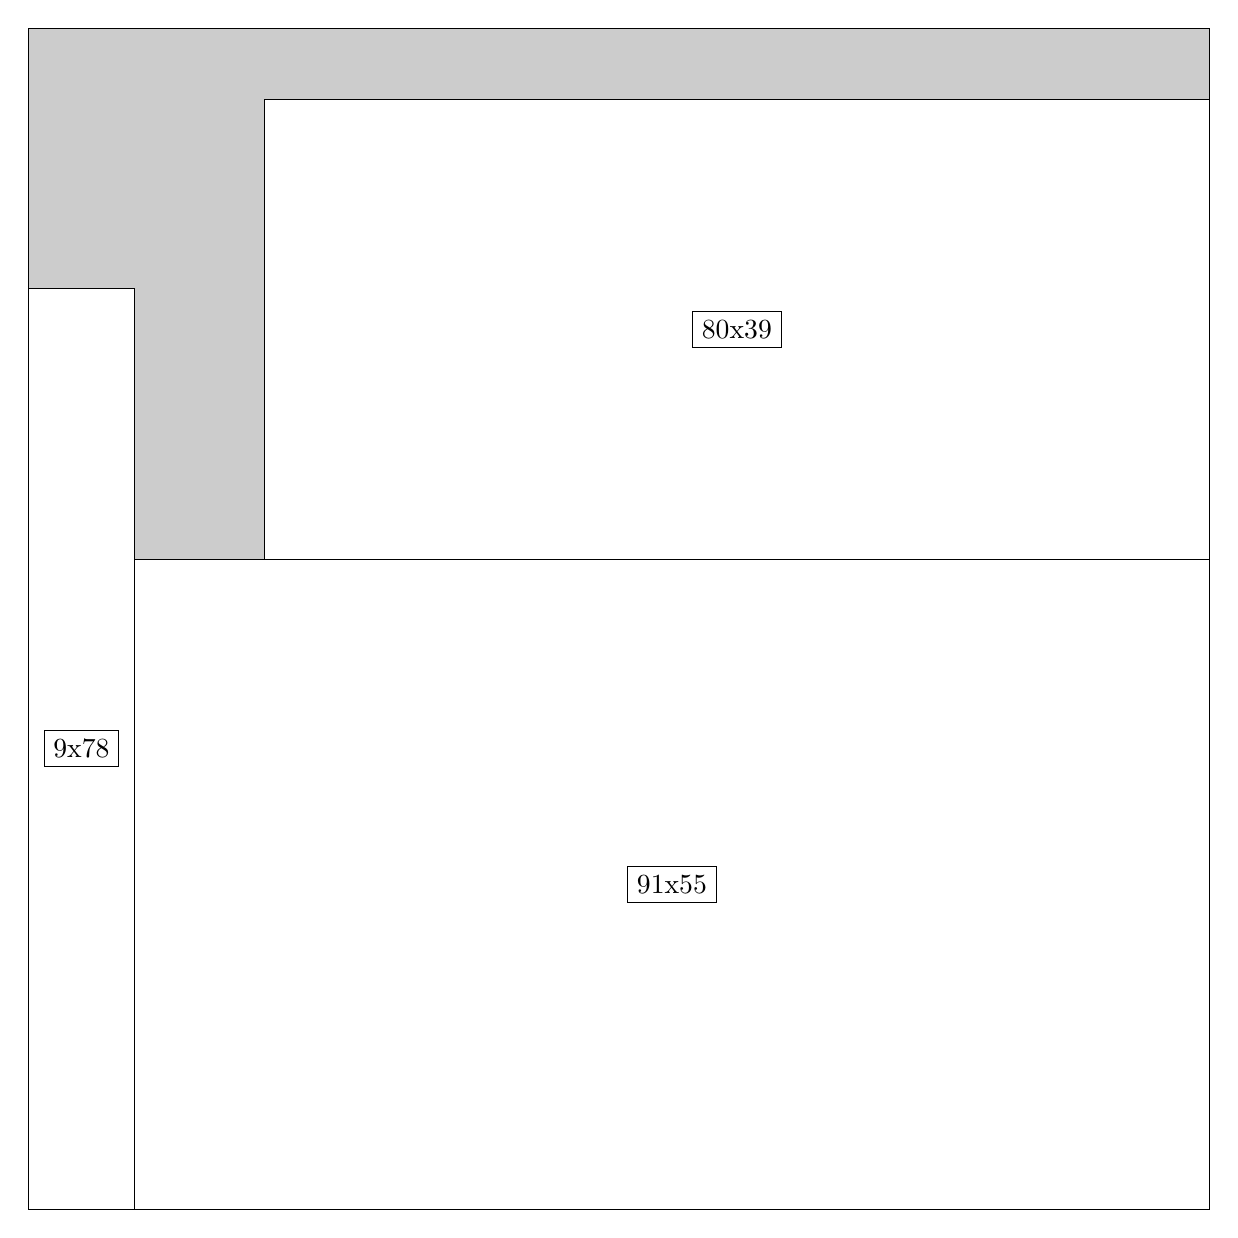
\begin{tikzpicture}[shorten >=1pt,scale=1.0,every node/.style={scale=1.0},->]
\tikzstyle{vertex}=[circle,fill=black!25,minimum size=14pt,inner sep=0pt]
\filldraw[fill=gray!40!white, draw=black] (0,0) rectangle (15.0,15.0);
\foreach \name/\x/\y/\w/\h in {91x55/1.3499999999999999/0.0/13.65/8.25,80x39/3.0/8.25/12.0/5.85,9x78/0.0/0.0/1.3499999999999999/11.7}
\filldraw[fill=white!40!white, draw=black] (\x,\y) rectangle node[draw] (\name) {\name} ++(\w,\h);
\end{tikzpicture}


w =91 , h =55 , x =9 , y =0 , v =5005
\par
w =80 , h =39 , x =20 , y =55 , v =3120
\par
w =9 , h =78 , x =0 , y =0 , v =702
\par
\newpage


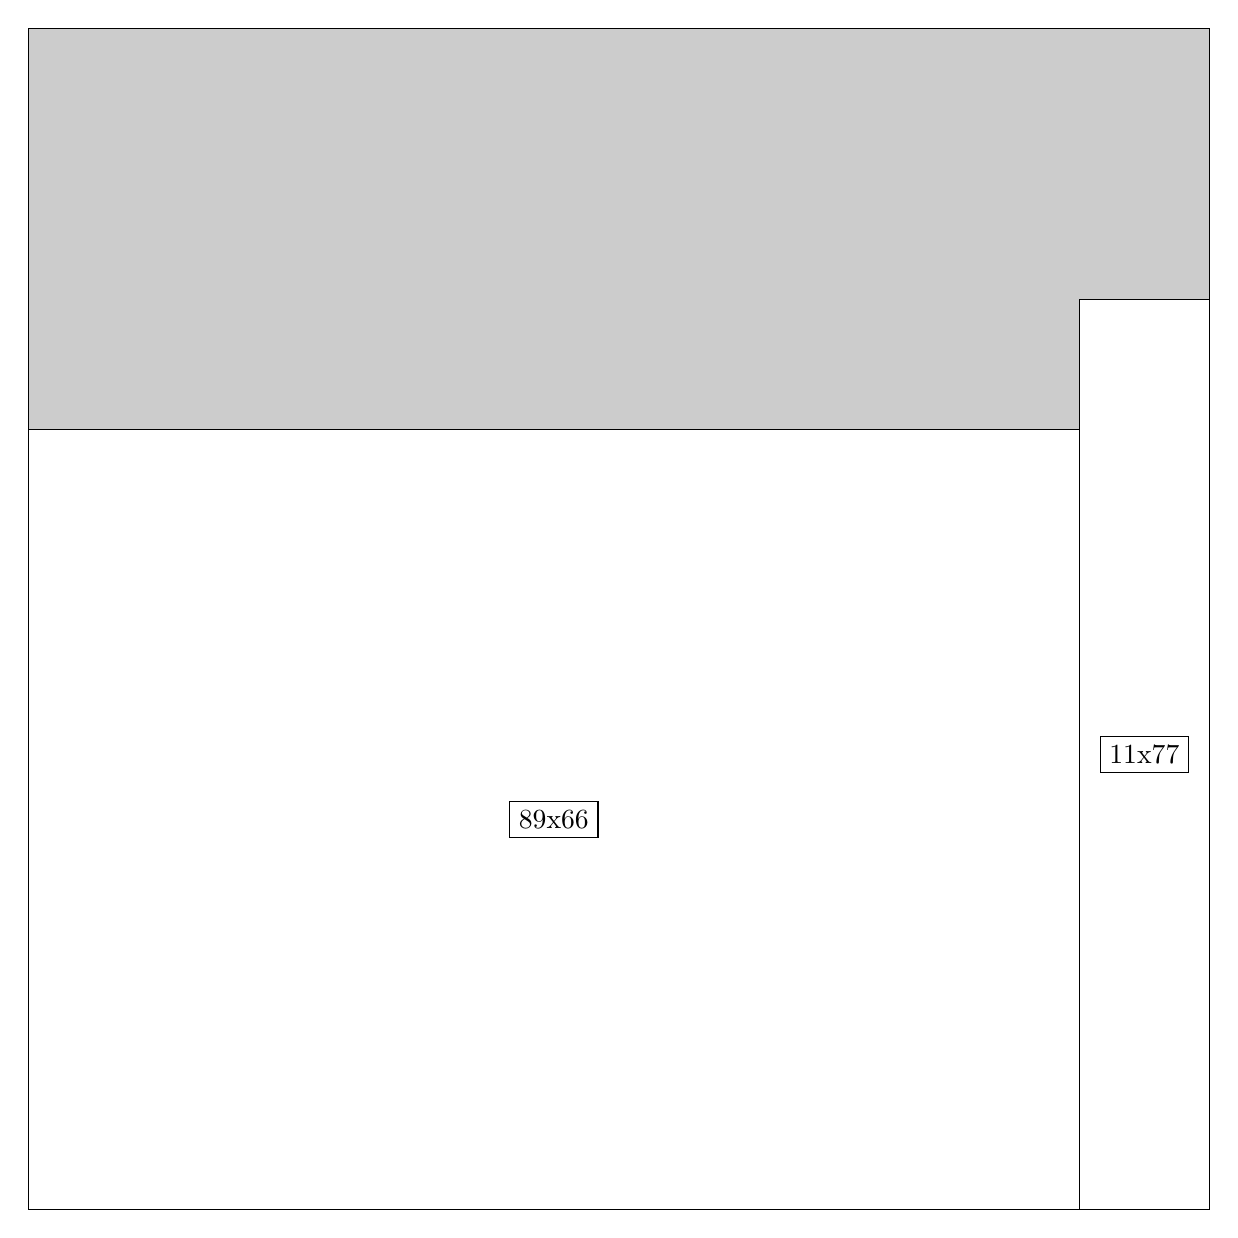
\begin{tikzpicture}[shorten >=1pt,scale=1.0,every node/.style={scale=1.0},->]
\tikzstyle{vertex}=[circle,fill=black!25,minimum size=14pt,inner sep=0pt]
\filldraw[fill=gray!40!white, draw=black] (0,0) rectangle (15.0,15.0);
\foreach \name/\x/\y/\w/\h in {11x77/13.35/0.0/1.65/11.549999999999999,89x66/0.0/0.0/13.35/9.9}
\filldraw[fill=white!40!white, draw=black] (\x,\y) rectangle node[draw] (\name) {\name} ++(\w,\h);
\end{tikzpicture}


w =11 , h =77 , x =89 , y =0 , v =847
\par
w =89 , h =66 , x =0 , y =0 , v =5874
\par
\newpage


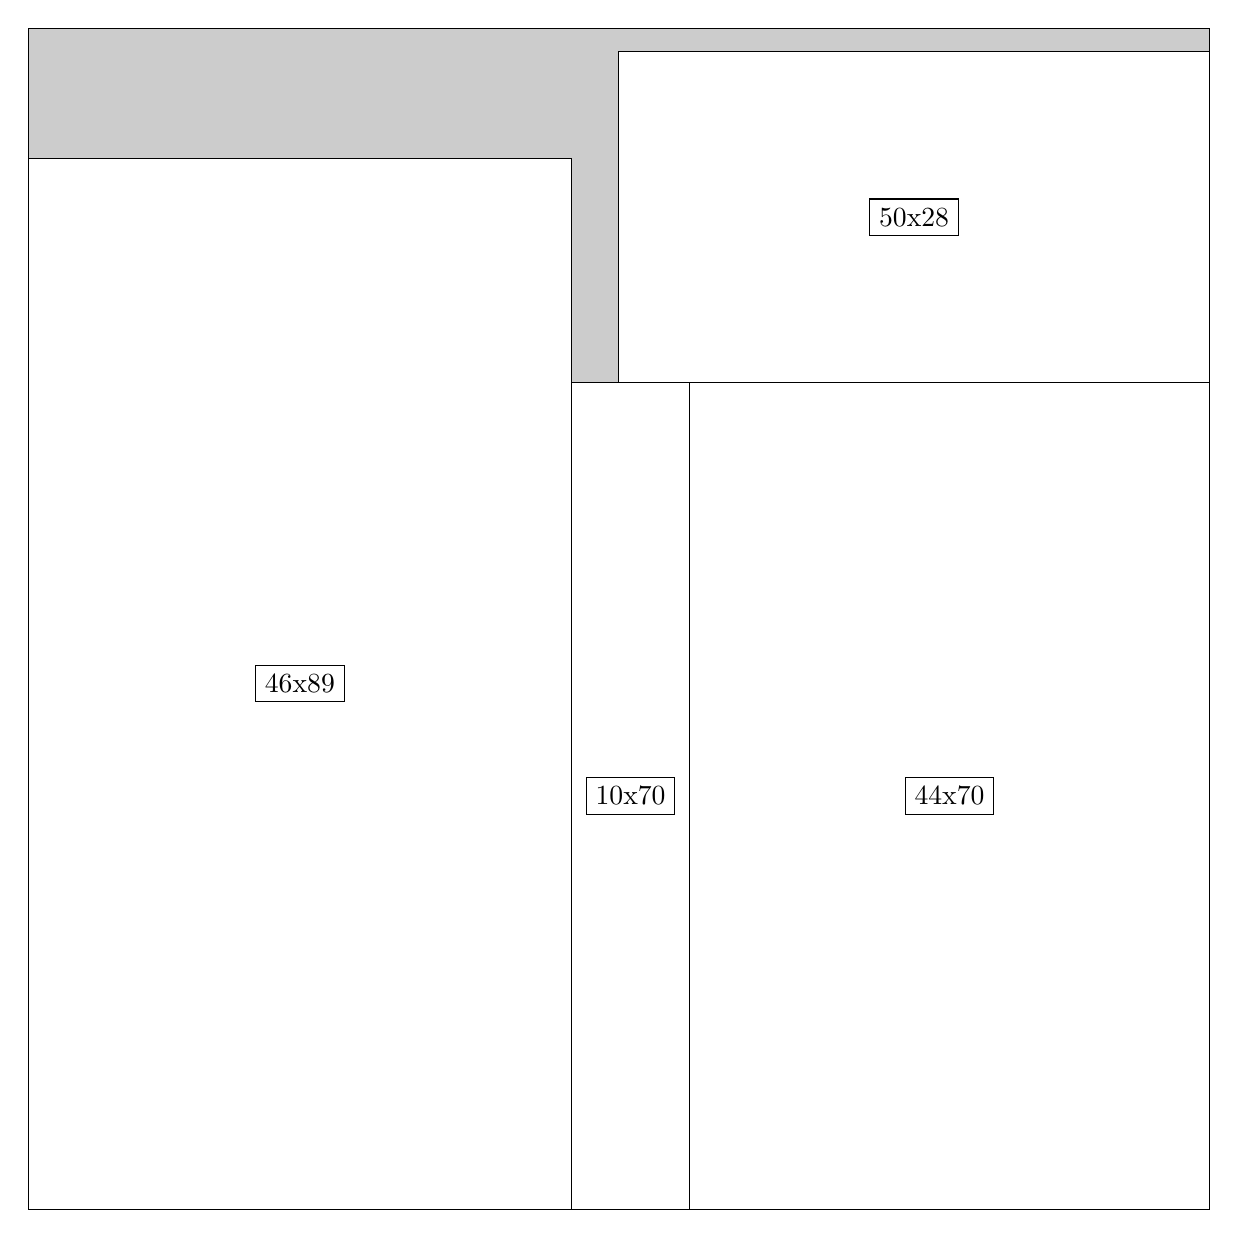
\begin{tikzpicture}[shorten >=1pt,scale=1.0,every node/.style={scale=1.0},->]
\tikzstyle{vertex}=[circle,fill=black!25,minimum size=14pt,inner sep=0pt]
\filldraw[fill=gray!40!white, draw=black] (0,0) rectangle (15.0,15.0);
\foreach \name/\x/\y/\w/\h in {44x70/8.4/0.0/6.6/10.5,10x70/6.8999999999999995/0.0/1.5/10.5,50x28/7.5/10.5/7.5/4.2,46x89/0.0/0.0/6.8999999999999995/13.35}
\filldraw[fill=white!40!white, draw=black] (\x,\y) rectangle node[draw] (\name) {\name} ++(\w,\h);
\end{tikzpicture}


w =44 , h =70 , x =56 , y =0 , v =3080
\par
w =10 , h =70 , x =46 , y =0 , v =700
\par
w =50 , h =28 , x =50 , y =70 , v =1400
\par
w =46 , h =89 , x =0 , y =0 , v =4094
\par
\newpage


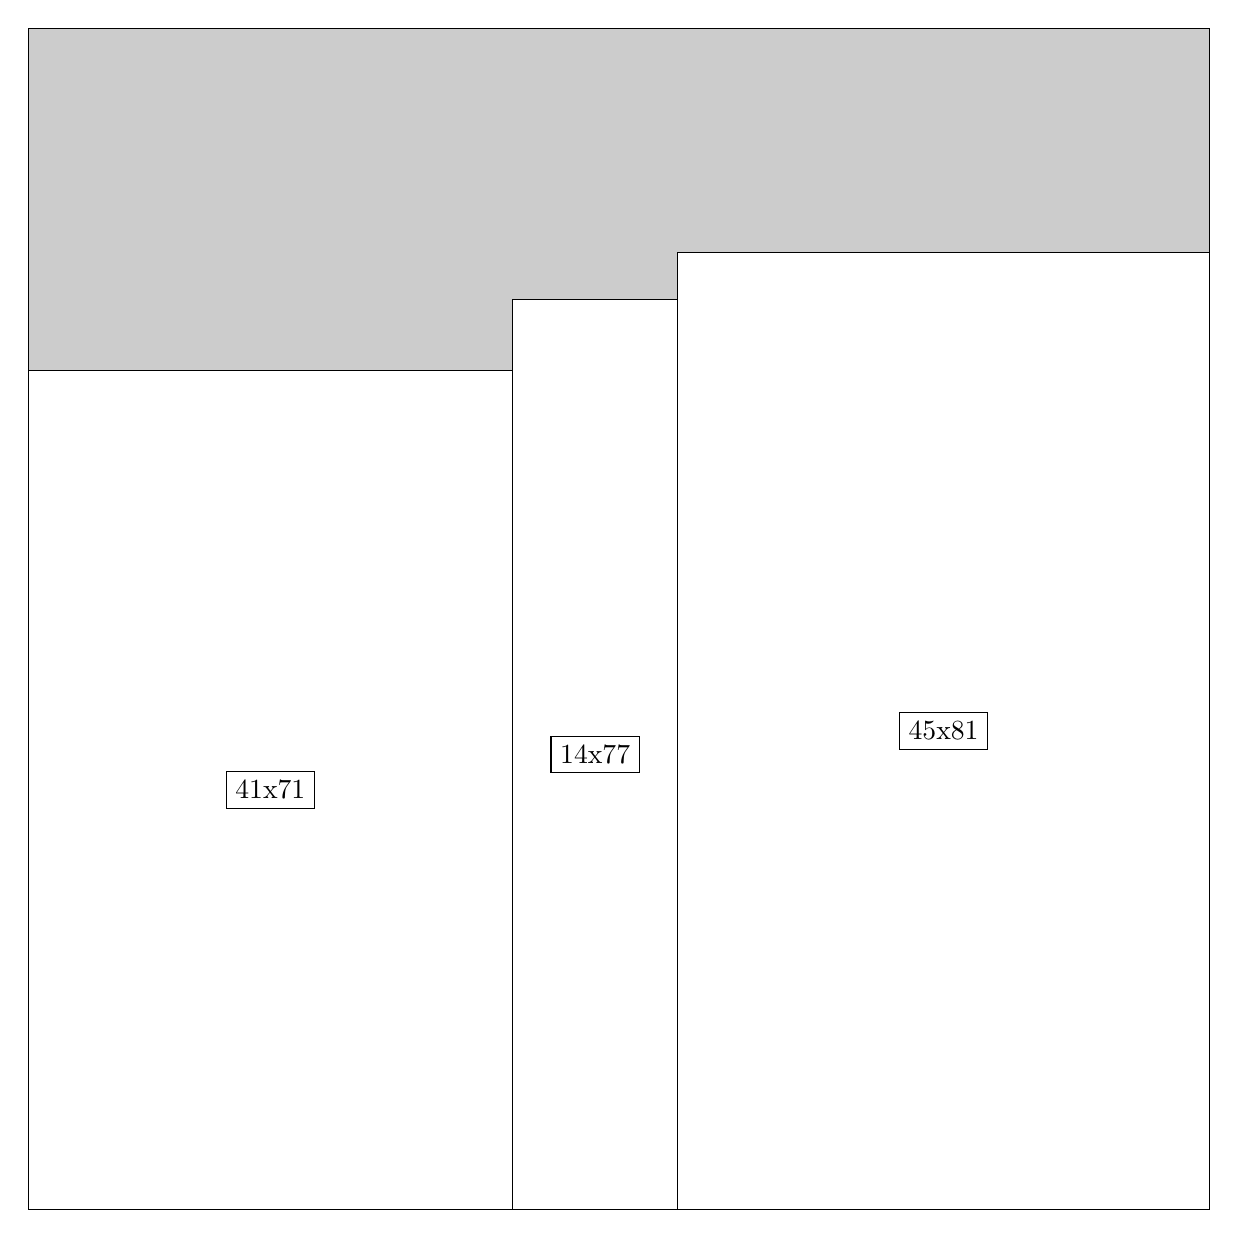
\begin{tikzpicture}[shorten >=1pt,scale=1.0,every node/.style={scale=1.0},->]
\tikzstyle{vertex}=[circle,fill=black!25,minimum size=14pt,inner sep=0pt]
\filldraw[fill=gray!40!white, draw=black] (0,0) rectangle (15.0,15.0);
\foreach \name/\x/\y/\w/\h in {45x81/8.25/0.0/6.75/12.15,14x77/6.1499999999999995/0.0/2.1/11.549999999999999,41x71/0.0/0.0/6.1499999999999995/10.65}
\filldraw[fill=white!40!white, draw=black] (\x,\y) rectangle node[draw] (\name) {\name} ++(\w,\h);
\end{tikzpicture}


w =45 , h =81 , x =55 , y =0 , v =3645
\par
w =14 , h =77 , x =41 , y =0 , v =1078
\par
w =41 , h =71 , x =0 , y =0 , v =2911
\par
\newpage


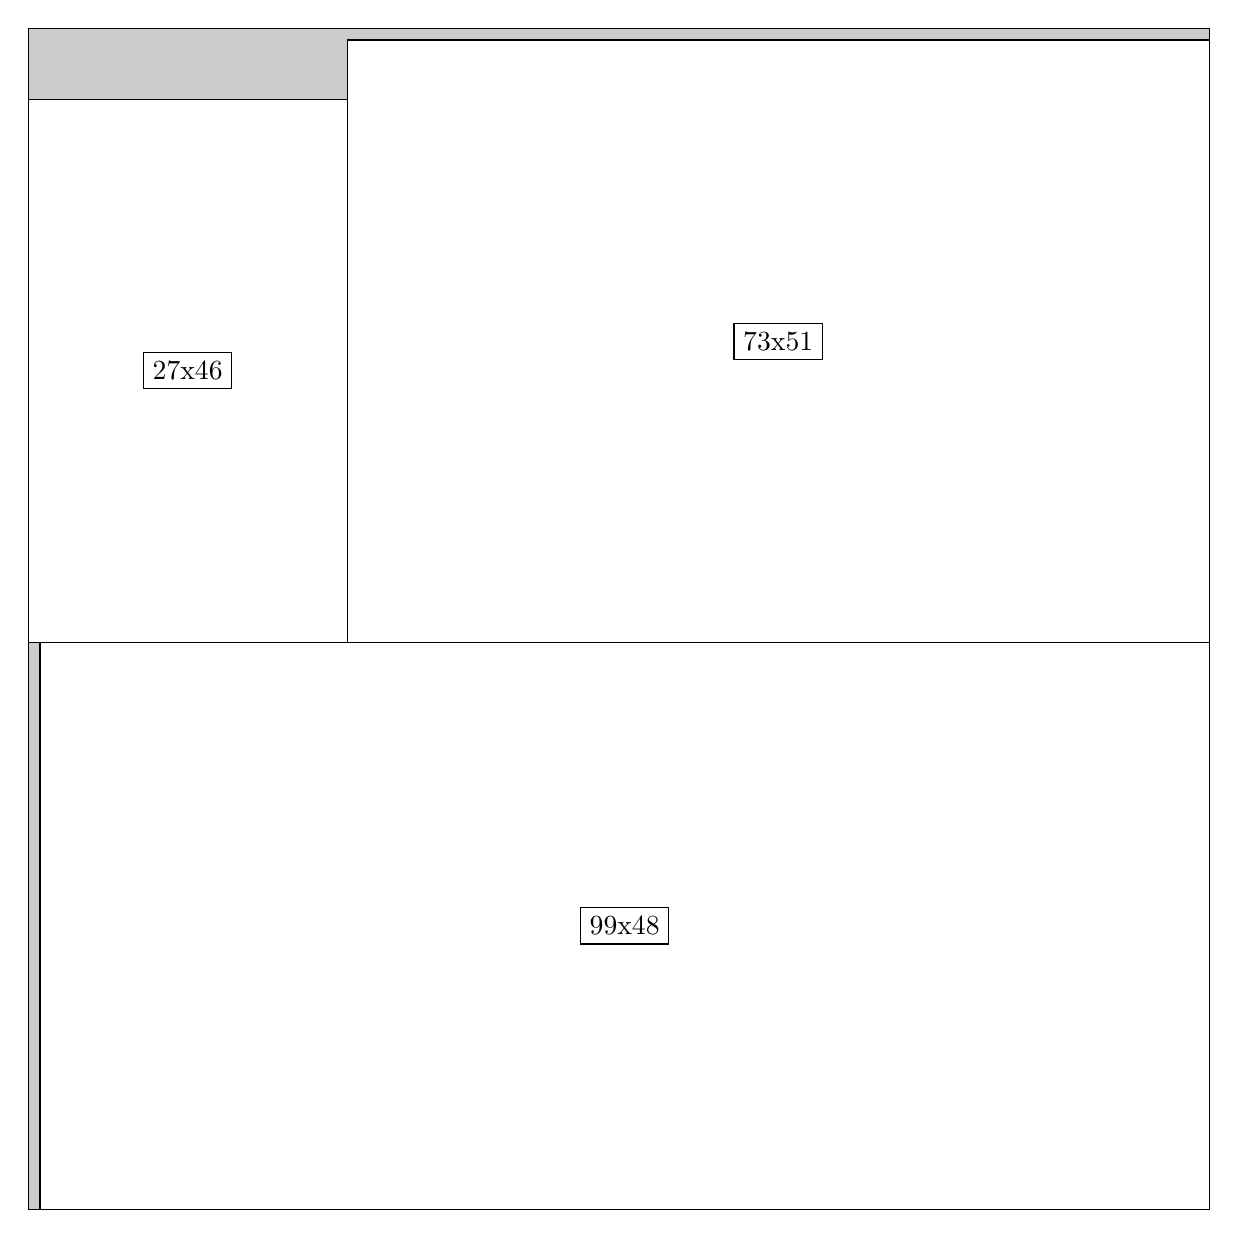
\begin{tikzpicture}[shorten >=1pt,scale=1.0,every node/.style={scale=1.0},->]
\tikzstyle{vertex}=[circle,fill=black!25,minimum size=14pt,inner sep=0pt]
\filldraw[fill=gray!40!white, draw=black] (0,0) rectangle (15.0,15.0);
\foreach \name/\x/\y/\w/\h in {99x48/0.15/0.0/14.85/7.199999999999999,73x51/4.05/7.199999999999999/10.95/7.6499999999999995,27x46/0.0/7.199999999999999/4.05/6.8999999999999995}
\filldraw[fill=white!40!white, draw=black] (\x,\y) rectangle node[draw] (\name) {\name} ++(\w,\h);
\end{tikzpicture}


w =99 , h =48 , x =1 , y =0 , v =4752
\par
w =73 , h =51 , x =27 , y =48 , v =3723
\par
w =27 , h =46 , x =0 , y =48 , v =1242
\par
\newpage


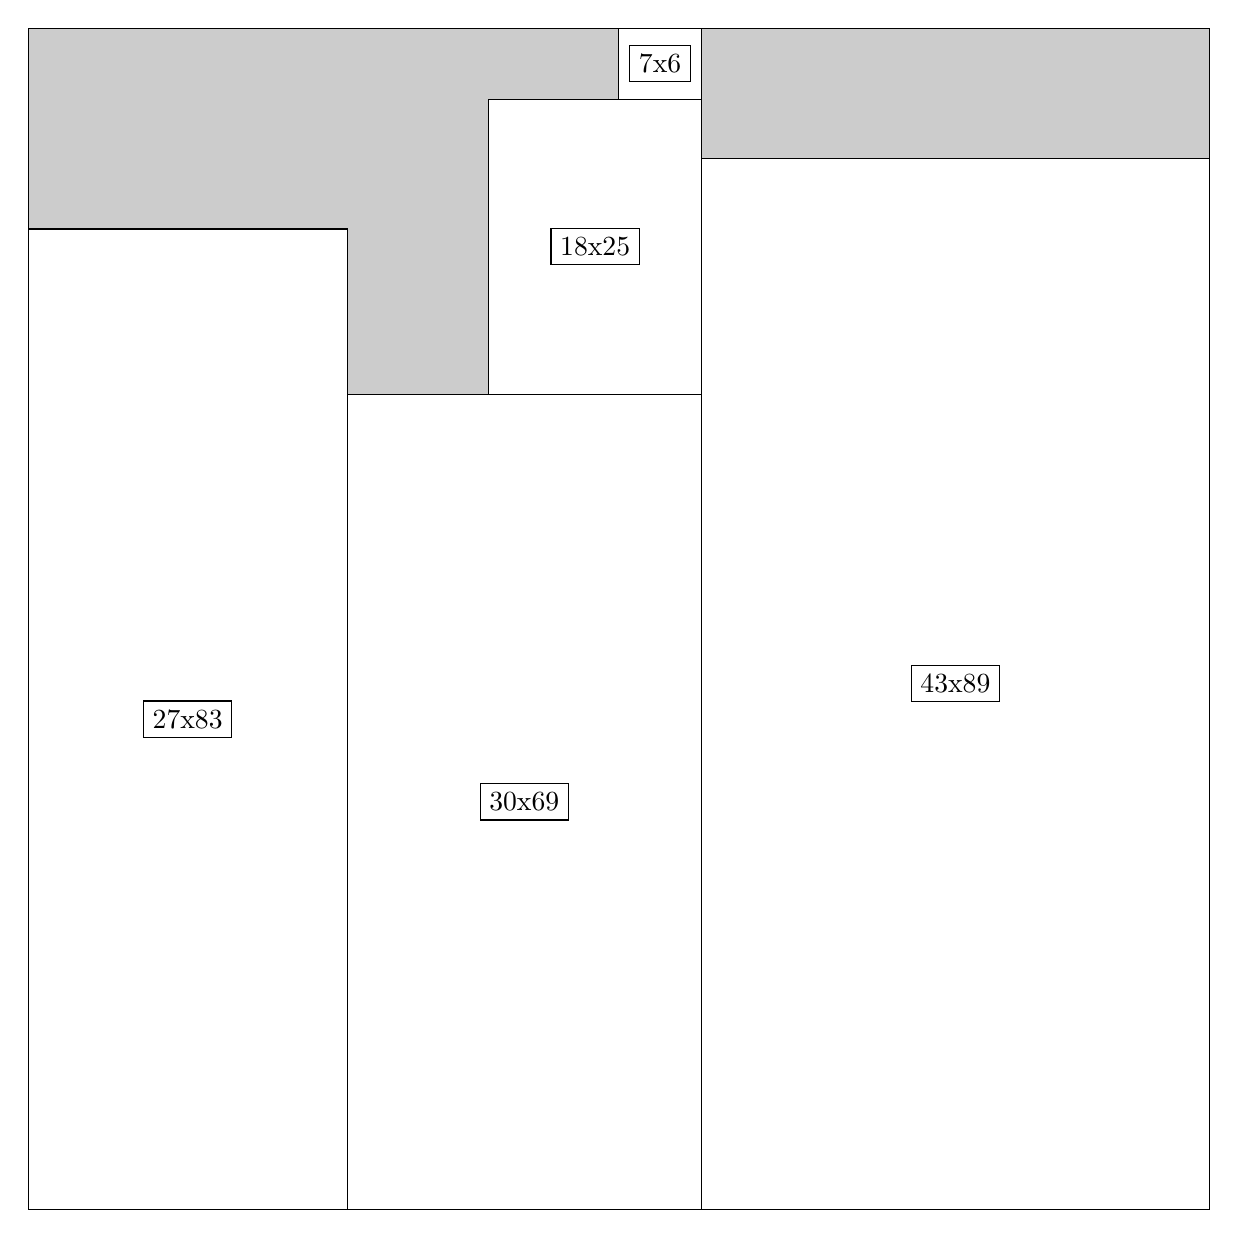
\begin{tikzpicture}[shorten >=1pt,scale=1.0,every node/.style={scale=1.0},->]
\tikzstyle{vertex}=[circle,fill=black!25,minimum size=14pt,inner sep=0pt]
\filldraw[fill=gray!40!white, draw=black] (0,0) rectangle (15.0,15.0);
\foreach \name/\x/\y/\w/\h in {43x89/8.549999999999999/0.0/6.45/13.35,30x69/4.05/0.0/4.5/10.35,18x25/5.85/10.35/2.6999999999999997/3.75,7x6/7.5/14.1/1.05/0.8999999999999999,27x83/0.0/0.0/4.05/12.45}
\filldraw[fill=white!40!white, draw=black] (\x,\y) rectangle node[draw] (\name) {\name} ++(\w,\h);
\end{tikzpicture}


w =43 , h =89 , x =57 , y =0 , v =3827
\par
w =30 , h =69 , x =27 , y =0 , v =2070
\par
w =18 , h =25 , x =39 , y =69 , v =450
\par
w =7 , h =6 , x =50 , y =94 , v =42
\par
w =27 , h =83 , x =0 , y =0 , v =2241
\par
\newpage


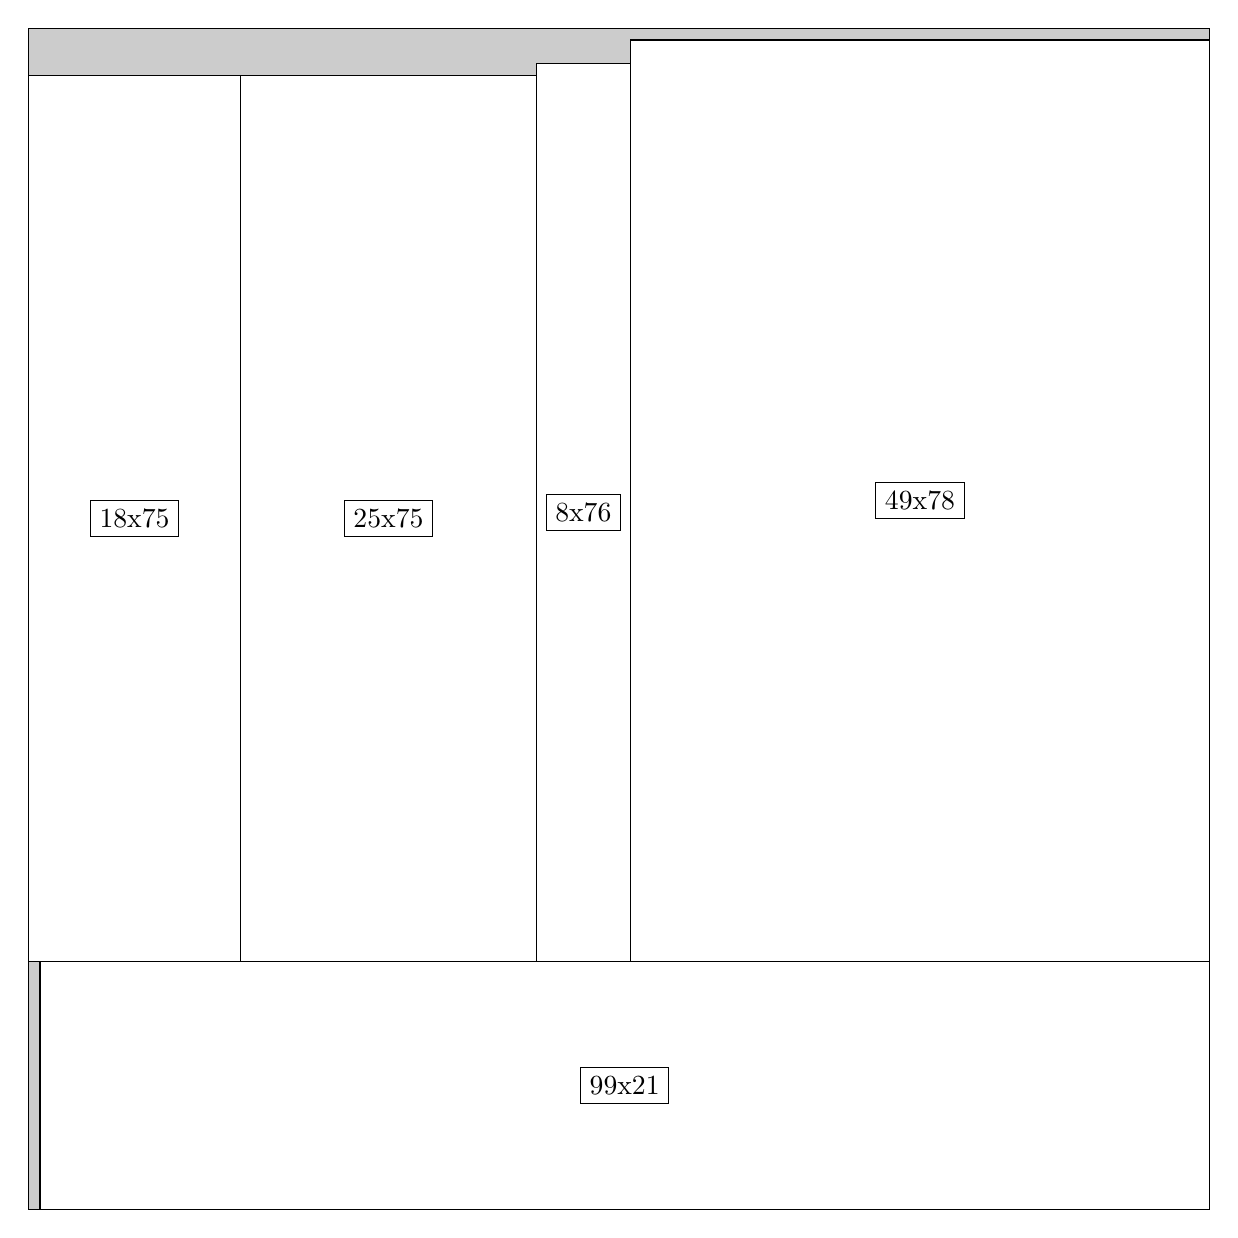
\begin{tikzpicture}[shorten >=1pt,scale=1.0,every node/.style={scale=1.0},->]
\tikzstyle{vertex}=[circle,fill=black!25,minimum size=14pt,inner sep=0pt]
\filldraw[fill=gray!40!white, draw=black] (0,0) rectangle (15.0,15.0);
\foreach \name/\x/\y/\w/\h in {99x21/0.15/0.0/14.85/3.15,49x78/7.6499999999999995/3.15/7.35/11.7,8x76/6.45/3.15/1.2/11.4,25x75/2.6999999999999997/3.15/3.75/11.25,18x75/0.0/3.15/2.6999999999999997/11.25}
\filldraw[fill=white!40!white, draw=black] (\x,\y) rectangle node[draw] (\name) {\name} ++(\w,\h);
\end{tikzpicture}


w =99 , h =21 , x =1 , y =0 , v =2079
\par
w =49 , h =78 , x =51 , y =21 , v =3822
\par
w =8 , h =76 , x =43 , y =21 , v =608
\par
w =25 , h =75 , x =18 , y =21 , v =1875
\par
w =18 , h =75 , x =0 , y =21 , v =1350
\par
\newpage


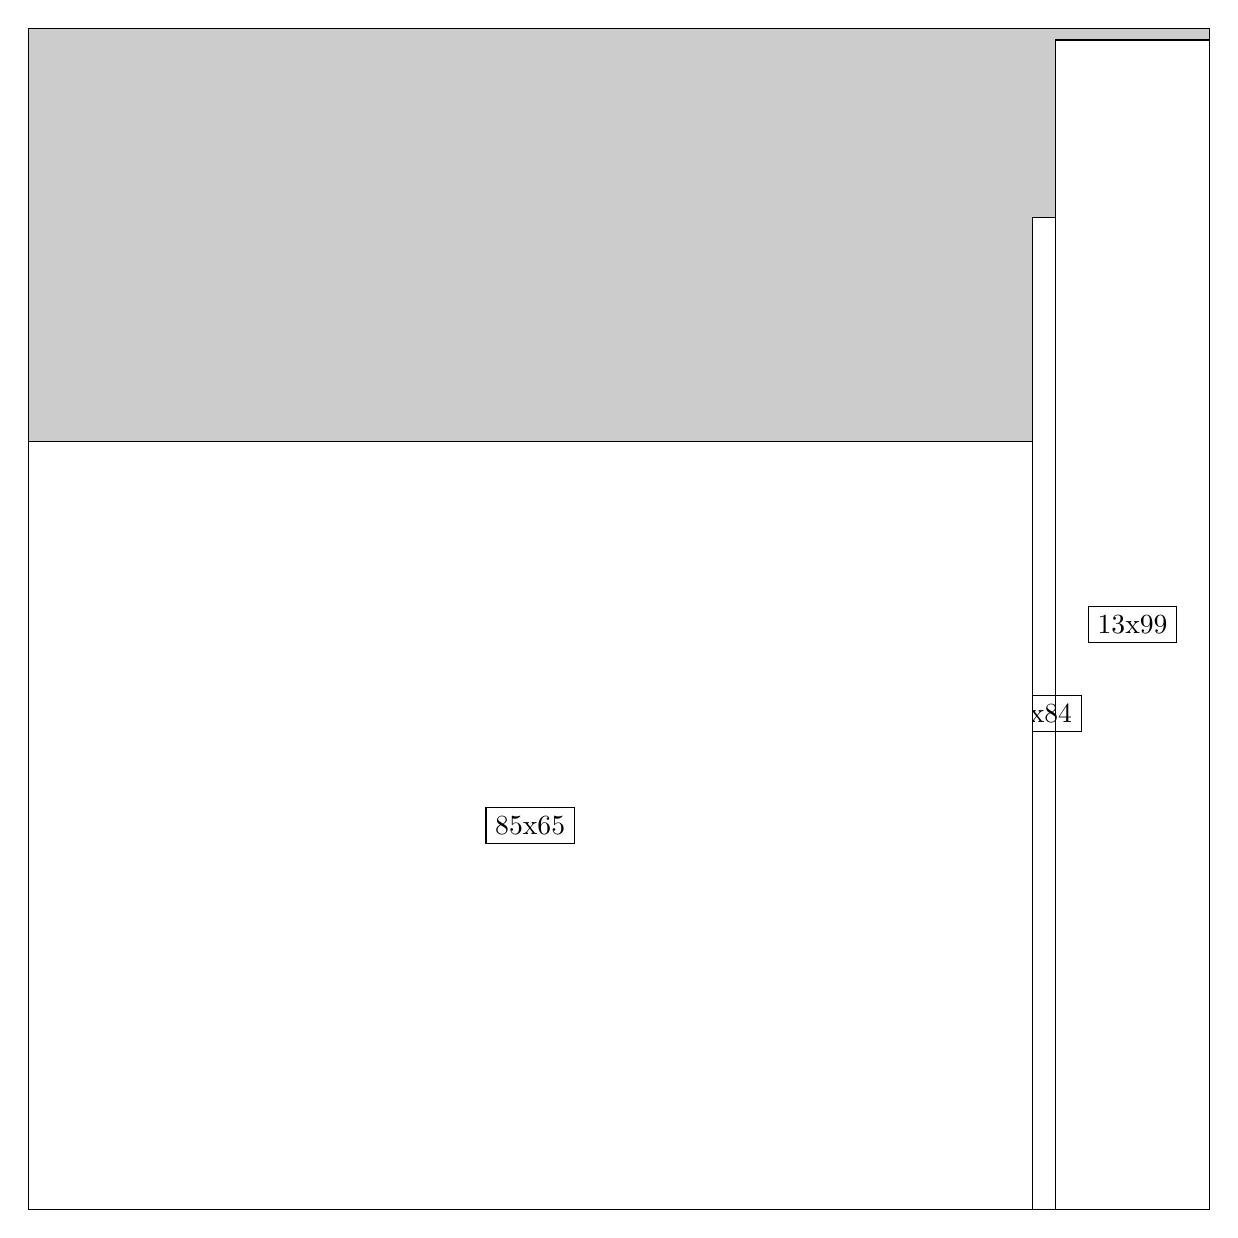
\begin{tikzpicture}[shorten >=1pt,scale=1.0,every node/.style={scale=1.0},->]
\tikzstyle{vertex}=[circle,fill=black!25,minimum size=14pt,inner sep=0pt]
\filldraw[fill=gray!40!white, draw=black] (0,0) rectangle (15.0,15.0);
\foreach \name/\x/\y/\w/\h in {13x99/13.049999999999999/0.0/1.95/14.85,2x84/12.75/0.0/0.3/12.6,85x65/0.0/0.0/12.75/9.75}
\filldraw[fill=white!40!white, draw=black] (\x,\y) rectangle node[draw] (\name) {\name} ++(\w,\h);
\end{tikzpicture}


w =13 , h =99 , x =87 , y =0 , v =1287
\par
w =2 , h =84 , x =85 , y =0 , v =168
\par
w =85 , h =65 , x =0 , y =0 , v =5525
\par
\newpage


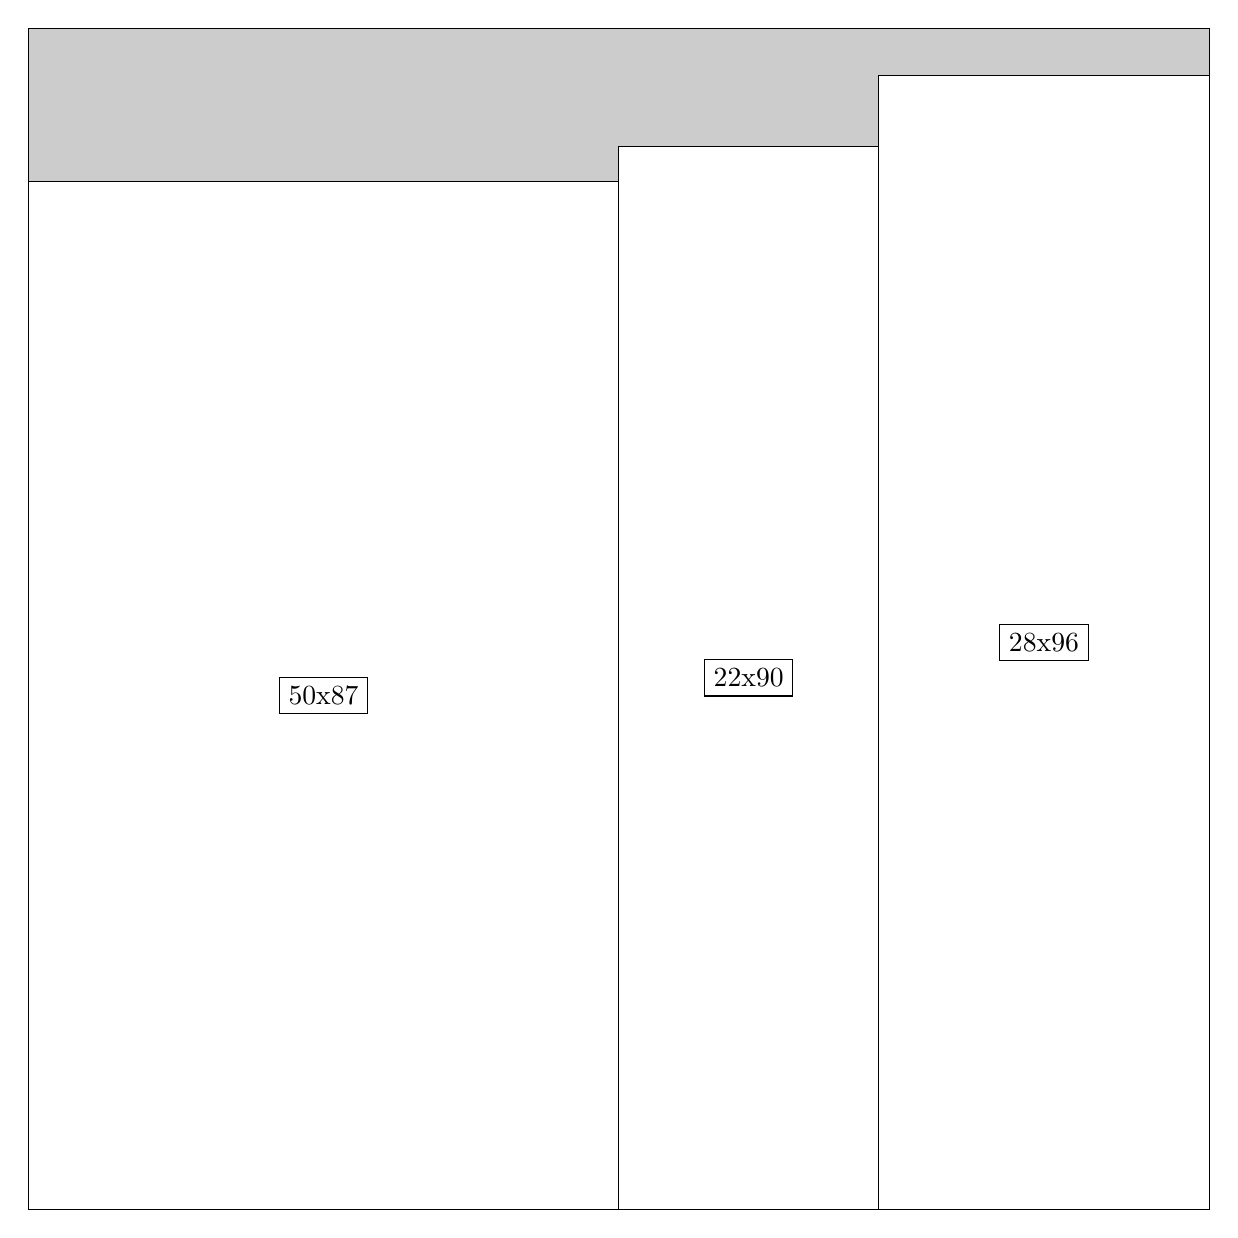
\begin{tikzpicture}[shorten >=1pt,scale=1.0,every node/.style={scale=1.0},->]
\tikzstyle{vertex}=[circle,fill=black!25,minimum size=14pt,inner sep=0pt]
\filldraw[fill=gray!40!white, draw=black] (0,0) rectangle (15.0,15.0);
\foreach \name/\x/\y/\w/\h in {28x96/10.799999999999999/0.0/4.2/14.399999999999999,22x90/7.5/0.0/3.3/13.5,50x87/0.0/0.0/7.5/13.049999999999999}
\filldraw[fill=white!40!white, draw=black] (\x,\y) rectangle node[draw] (\name) {\name} ++(\w,\h);
\end{tikzpicture}


w =28 , h =96 , x =72 , y =0 , v =2688
\par
w =22 , h =90 , x =50 , y =0 , v =1980
\par
w =50 , h =87 , x =0 , y =0 , v =4350
\par
\newpage


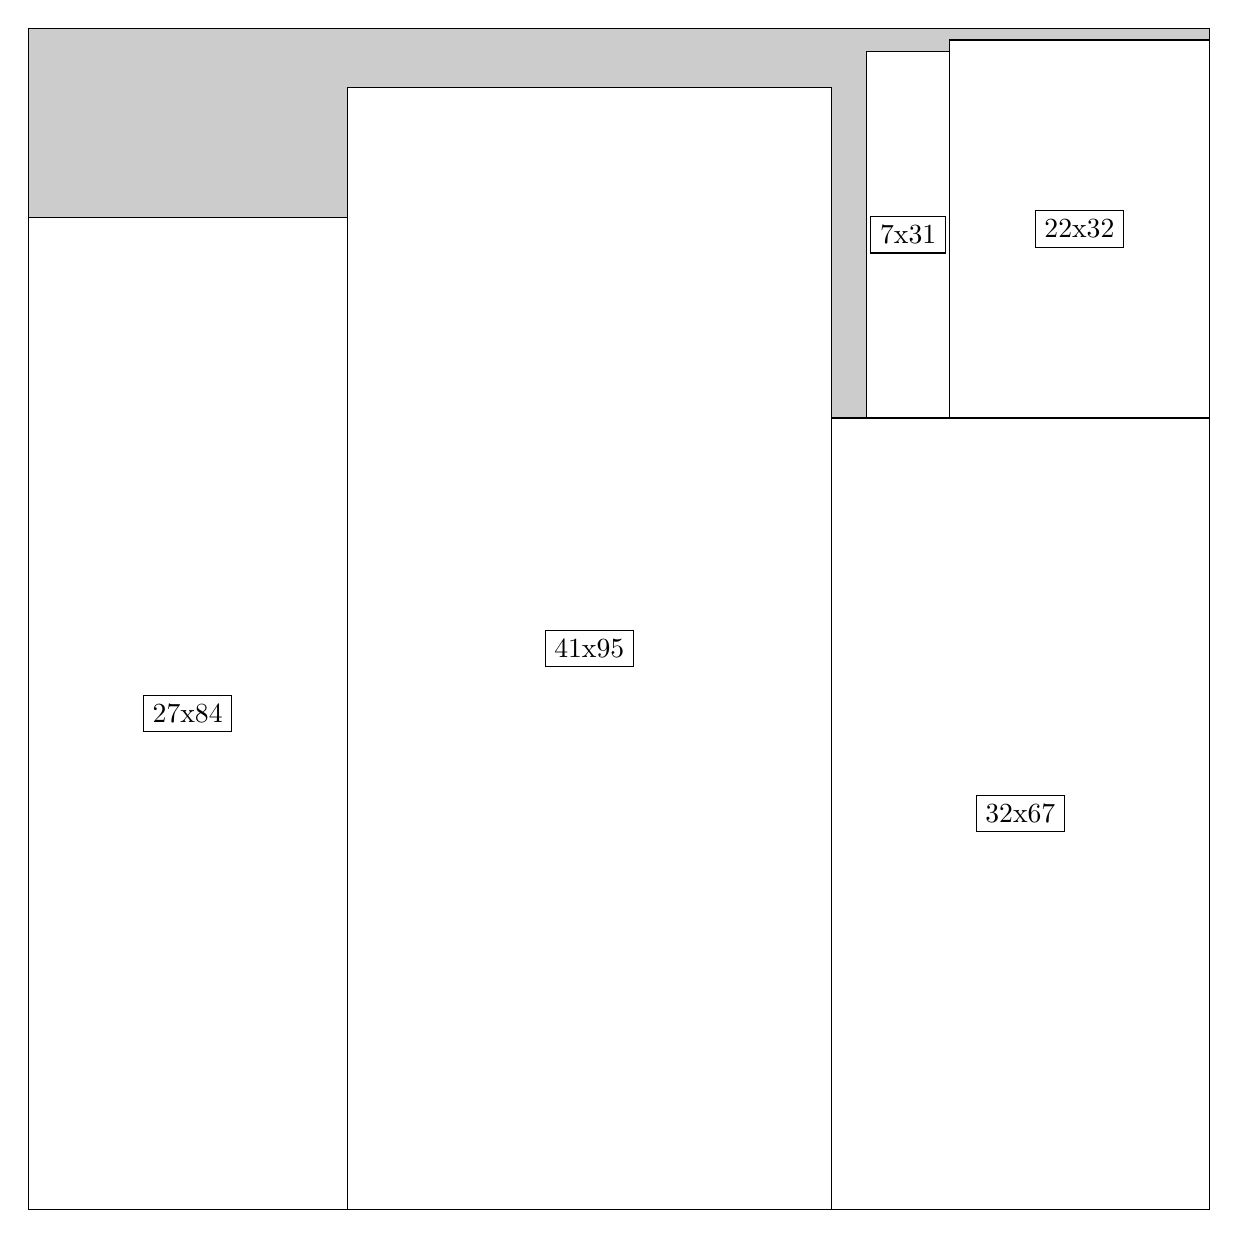
\begin{tikzpicture}[shorten >=1pt,scale=1.0,every node/.style={scale=1.0},->]
\tikzstyle{vertex}=[circle,fill=black!25,minimum size=14pt,inner sep=0pt]
\filldraw[fill=gray!40!white, draw=black] (0,0) rectangle (15.0,15.0);
\foreach \name/\x/\y/\w/\h in {32x67/10.2/0.0/4.8/10.049999999999999,22x32/11.7/10.049999999999999/3.3/4.8,7x31/10.65/10.049999999999999/1.05/4.6499999999999995,41x95/4.05/0.0/6.1499999999999995/14.25,27x84/0.0/0.0/4.05/12.6}
\filldraw[fill=white!40!white, draw=black] (\x,\y) rectangle node[draw] (\name) {\name} ++(\w,\h);
\end{tikzpicture}


w =32 , h =67 , x =68 , y =0 , v =2144
\par
w =22 , h =32 , x =78 , y =67 , v =704
\par
w =7 , h =31 , x =71 , y =67 , v =217
\par
w =41 , h =95 , x =27 , y =0 , v =3895
\par
w =27 , h =84 , x =0 , y =0 , v =2268
\par
\newpage


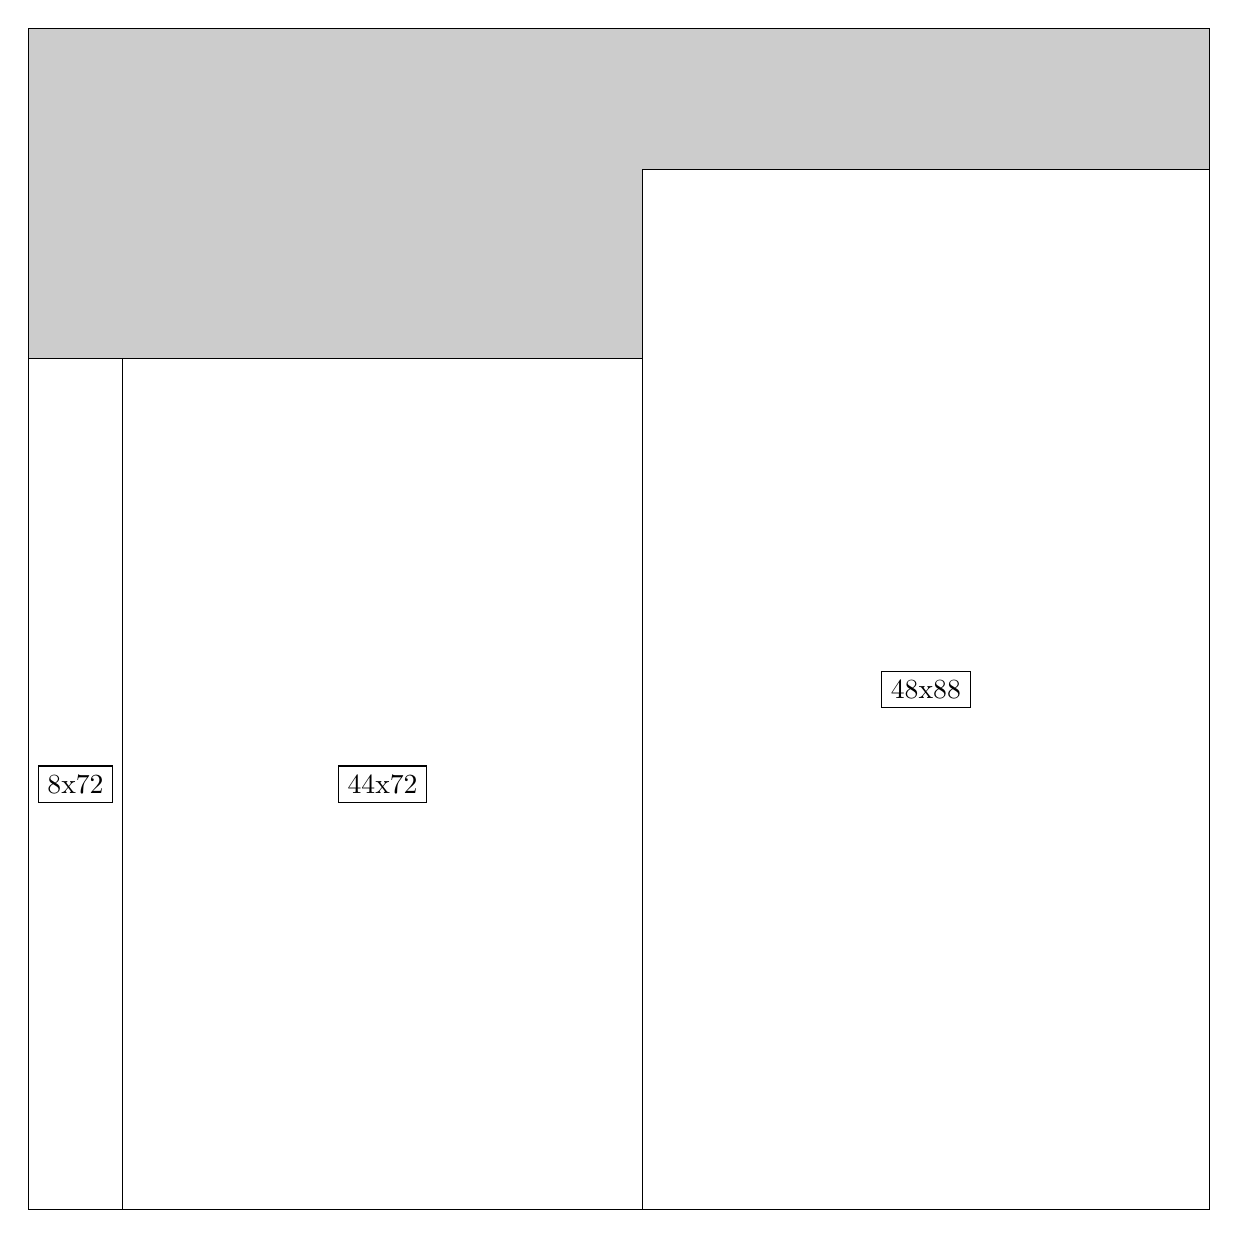
\begin{tikzpicture}[shorten >=1pt,scale=1.0,every node/.style={scale=1.0},->]
\tikzstyle{vertex}=[circle,fill=black!25,minimum size=14pt,inner sep=0pt]
\filldraw[fill=gray!40!white, draw=black] (0,0) rectangle (15.0,15.0);
\foreach \name/\x/\y/\w/\h in {48x88/7.8/0.0/7.199999999999999/13.2,44x72/1.2/0.0/6.6/10.799999999999999,8x72/0.0/0.0/1.2/10.799999999999999}
\filldraw[fill=white!40!white, draw=black] (\x,\y) rectangle node[draw] (\name) {\name} ++(\w,\h);
\end{tikzpicture}


w =48 , h =88 , x =52 , y =0 , v =4224
\par
w =44 , h =72 , x =8 , y =0 , v =3168
\par
w =8 , h =72 , x =0 , y =0 , v =576
\par
\newpage


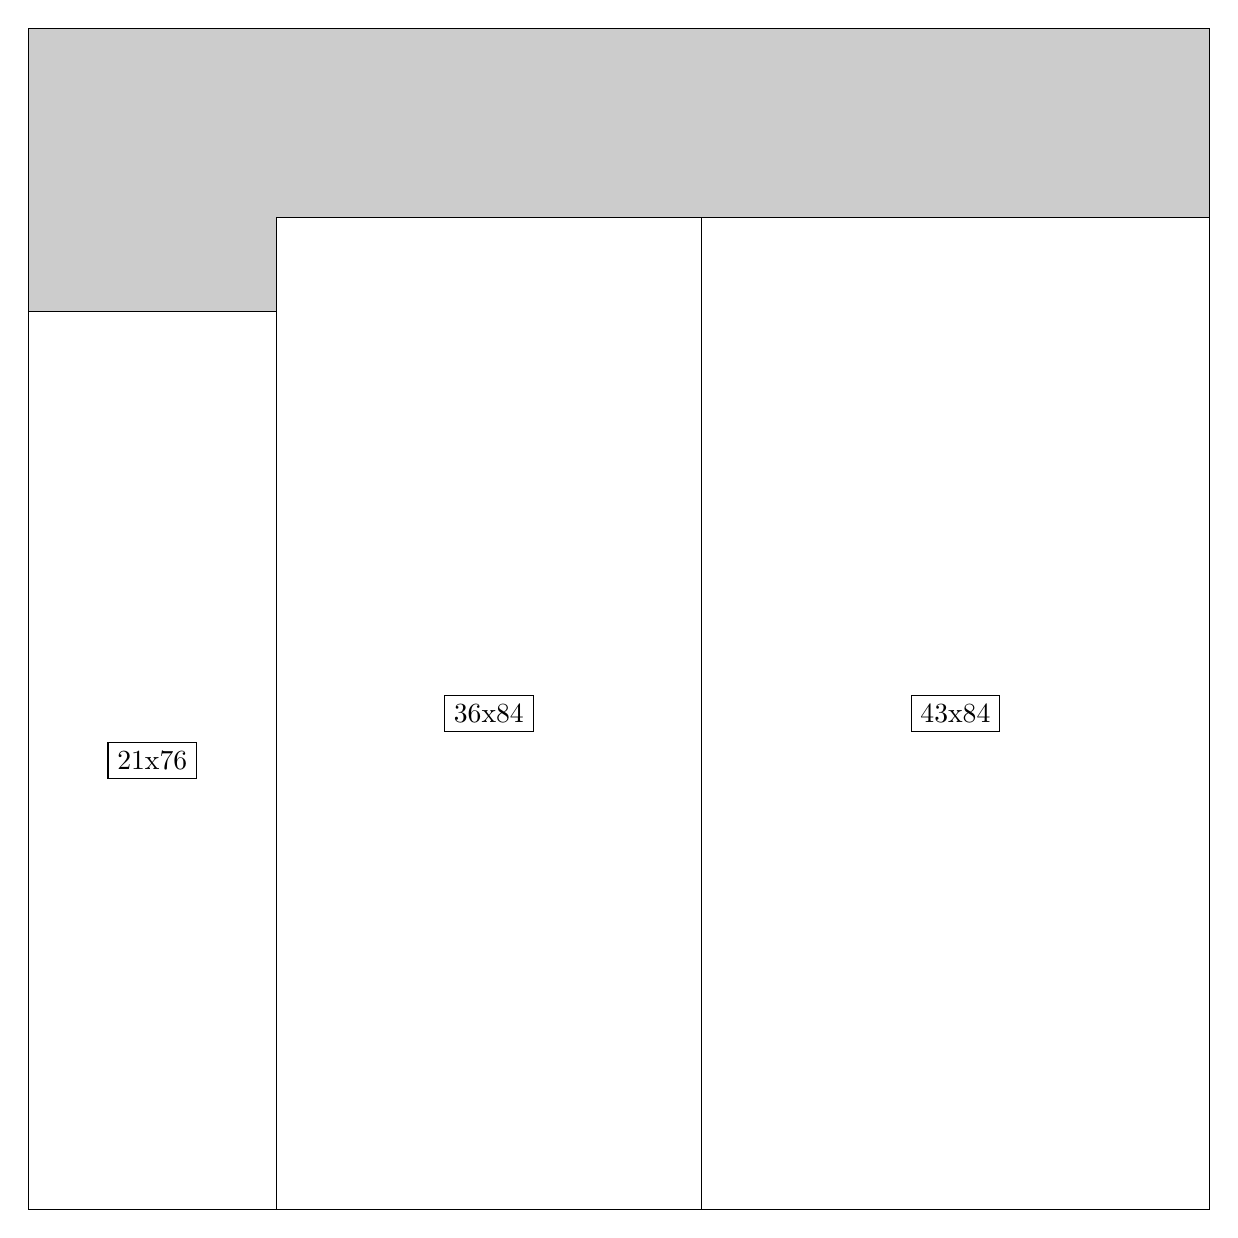
\begin{tikzpicture}[shorten >=1pt,scale=1.0,every node/.style={scale=1.0},->]
\tikzstyle{vertex}=[circle,fill=black!25,minimum size=14pt,inner sep=0pt]
\filldraw[fill=gray!40!white, draw=black] (0,0) rectangle (15.0,15.0);
\foreach \name/\x/\y/\w/\h in {43x84/8.549999999999999/0.0/6.45/12.6,36x84/3.15/0.0/5.3999999999999995/12.6,21x76/0.0/0.0/3.15/11.4}
\filldraw[fill=white!40!white, draw=black] (\x,\y) rectangle node[draw] (\name) {\name} ++(\w,\h);
\end{tikzpicture}


w =43 , h =84 , x =57 , y =0 , v =3612
\par
w =36 , h =84 , x =21 , y =0 , v =3024
\par
w =21 , h =76 , x =0 , y =0 , v =1596
\par
\newpage


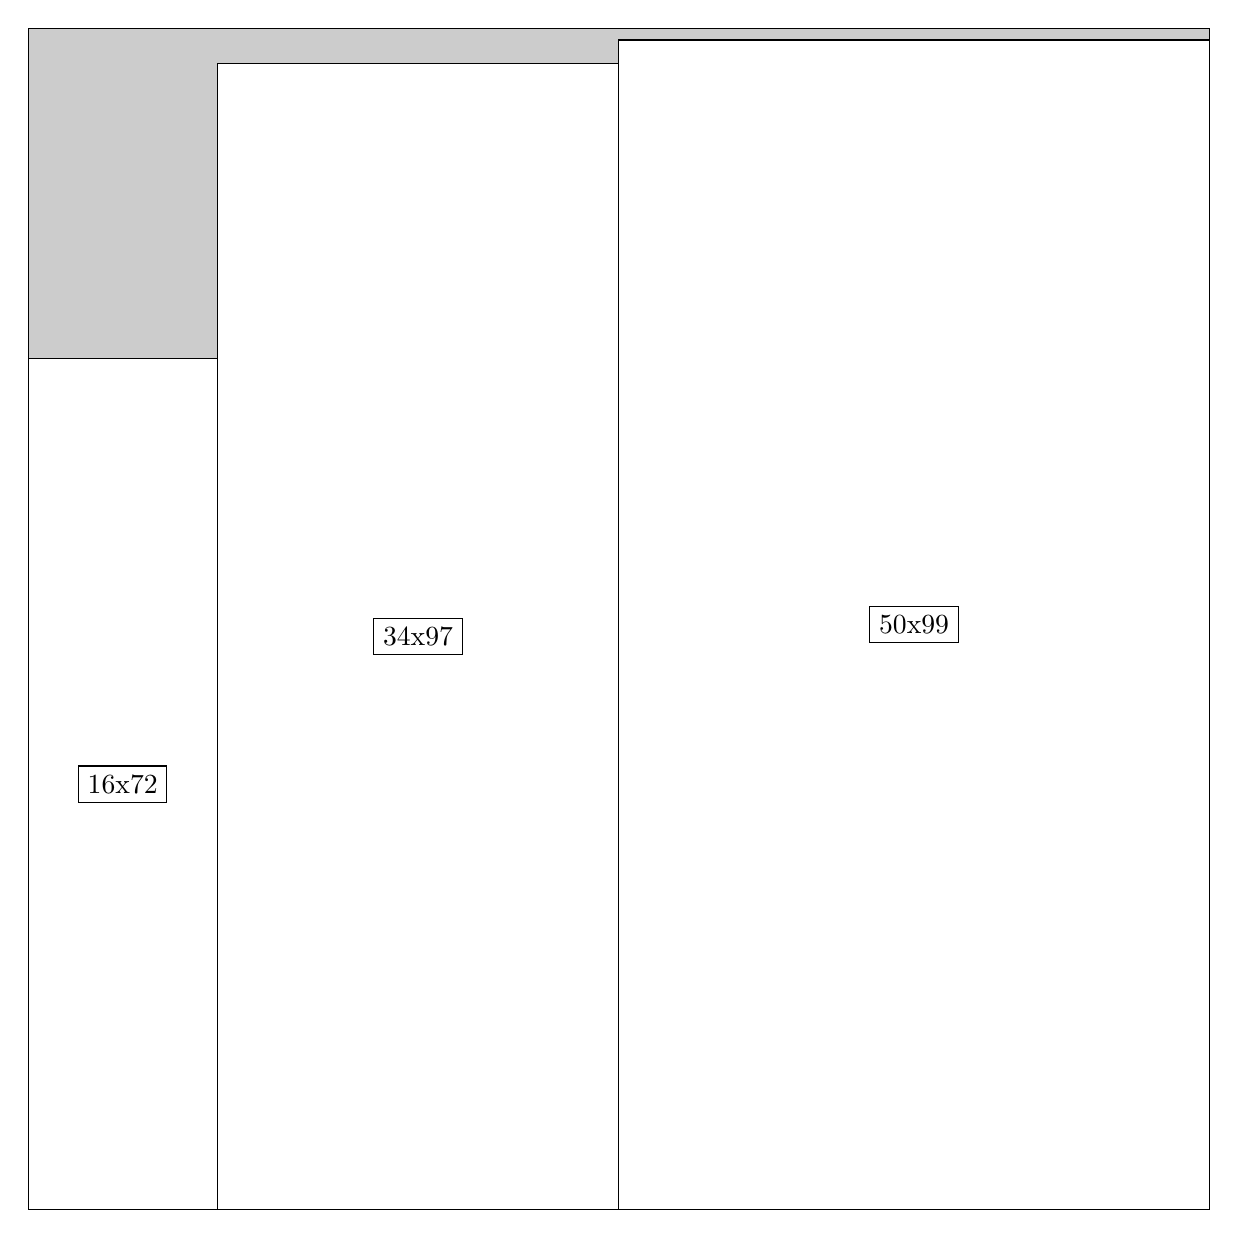
\begin{tikzpicture}[shorten >=1pt,scale=1.0,every node/.style={scale=1.0},->]
\tikzstyle{vertex}=[circle,fill=black!25,minimum size=14pt,inner sep=0pt]
\filldraw[fill=gray!40!white, draw=black] (0,0) rectangle (15.0,15.0);
\foreach \name/\x/\y/\w/\h in {50x99/7.5/0.0/7.5/14.85,34x97/2.4/0.0/5.1/14.549999999999999,16x72/0.0/0.0/2.4/10.799999999999999}
\filldraw[fill=white!40!white, draw=black] (\x,\y) rectangle node[draw] (\name) {\name} ++(\w,\h);
\end{tikzpicture}


w =50 , h =99 , x =50 , y =0 , v =4950
\par
w =34 , h =97 , x =16 , y =0 , v =3298
\par
w =16 , h =72 , x =0 , y =0 , v =1152
\par
\newpage


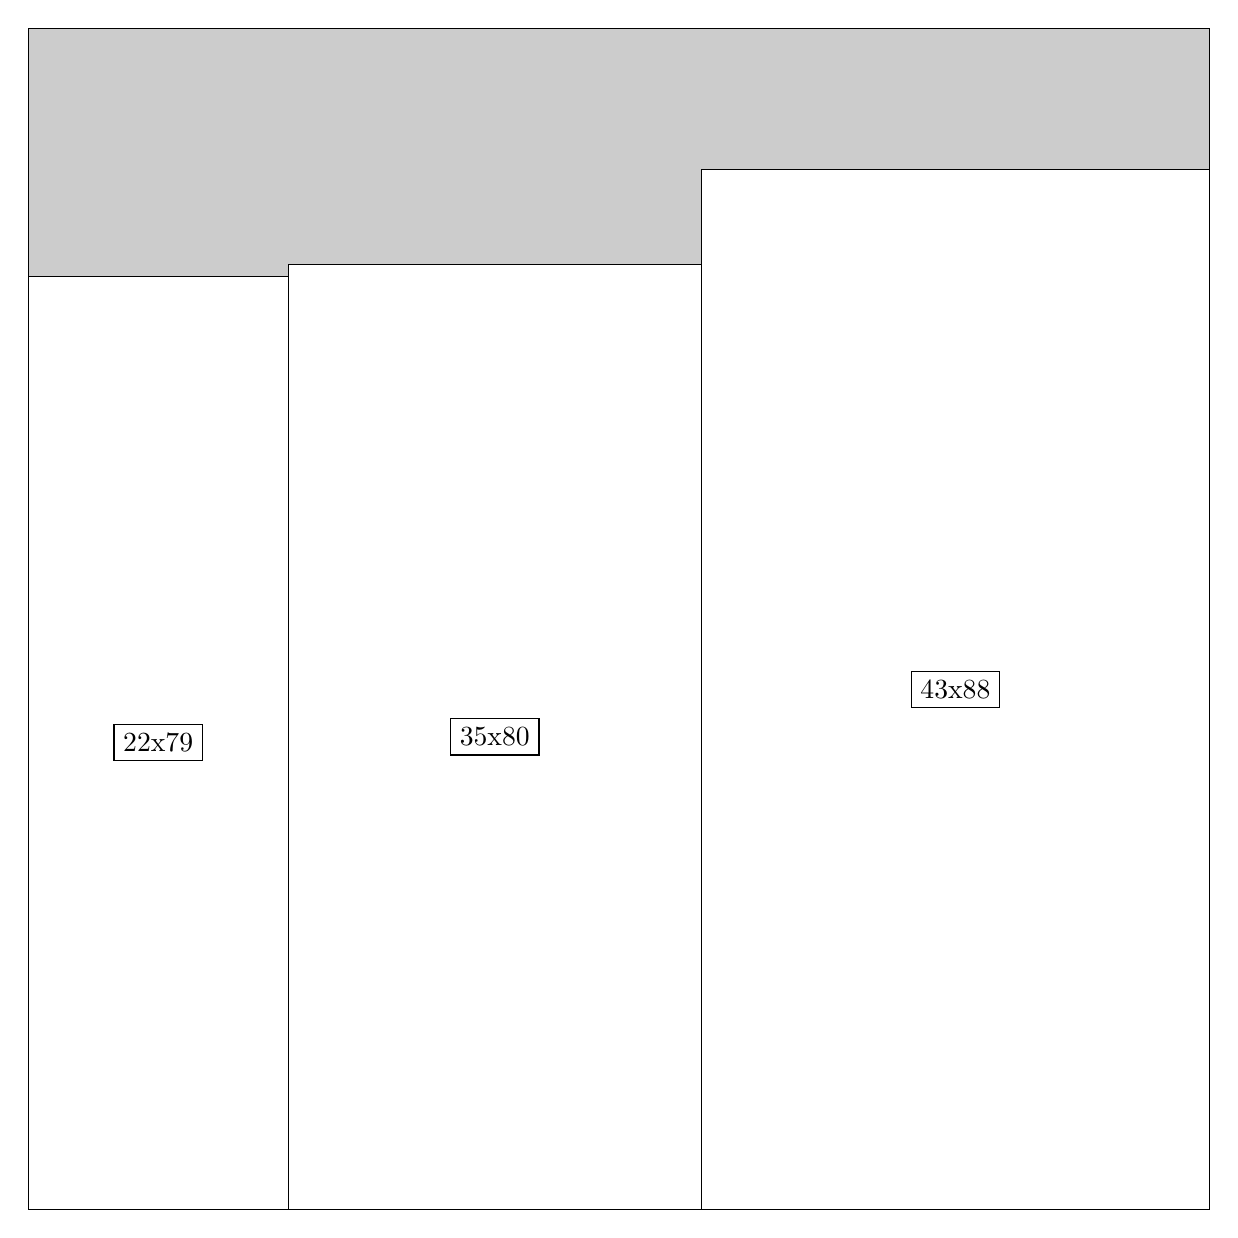
\begin{tikzpicture}[shorten >=1pt,scale=1.0,every node/.style={scale=1.0},->]
\tikzstyle{vertex}=[circle,fill=black!25,minimum size=14pt,inner sep=0pt]
\filldraw[fill=gray!40!white, draw=black] (0,0) rectangle (15.0,15.0);
\foreach \name/\x/\y/\w/\h in {43x88/8.549999999999999/0.0/6.45/13.2,35x80/3.3/0.0/5.25/12.0,22x79/0.0/0.0/3.3/11.85}
\filldraw[fill=white!40!white, draw=black] (\x,\y) rectangle node[draw] (\name) {\name} ++(\w,\h);
\end{tikzpicture}


w =43 , h =88 , x =57 , y =0 , v =3784
\par
w =35 , h =80 , x =22 , y =0 , v =2800
\par
w =22 , h =79 , x =0 , y =0 , v =1738
\par
\newpage


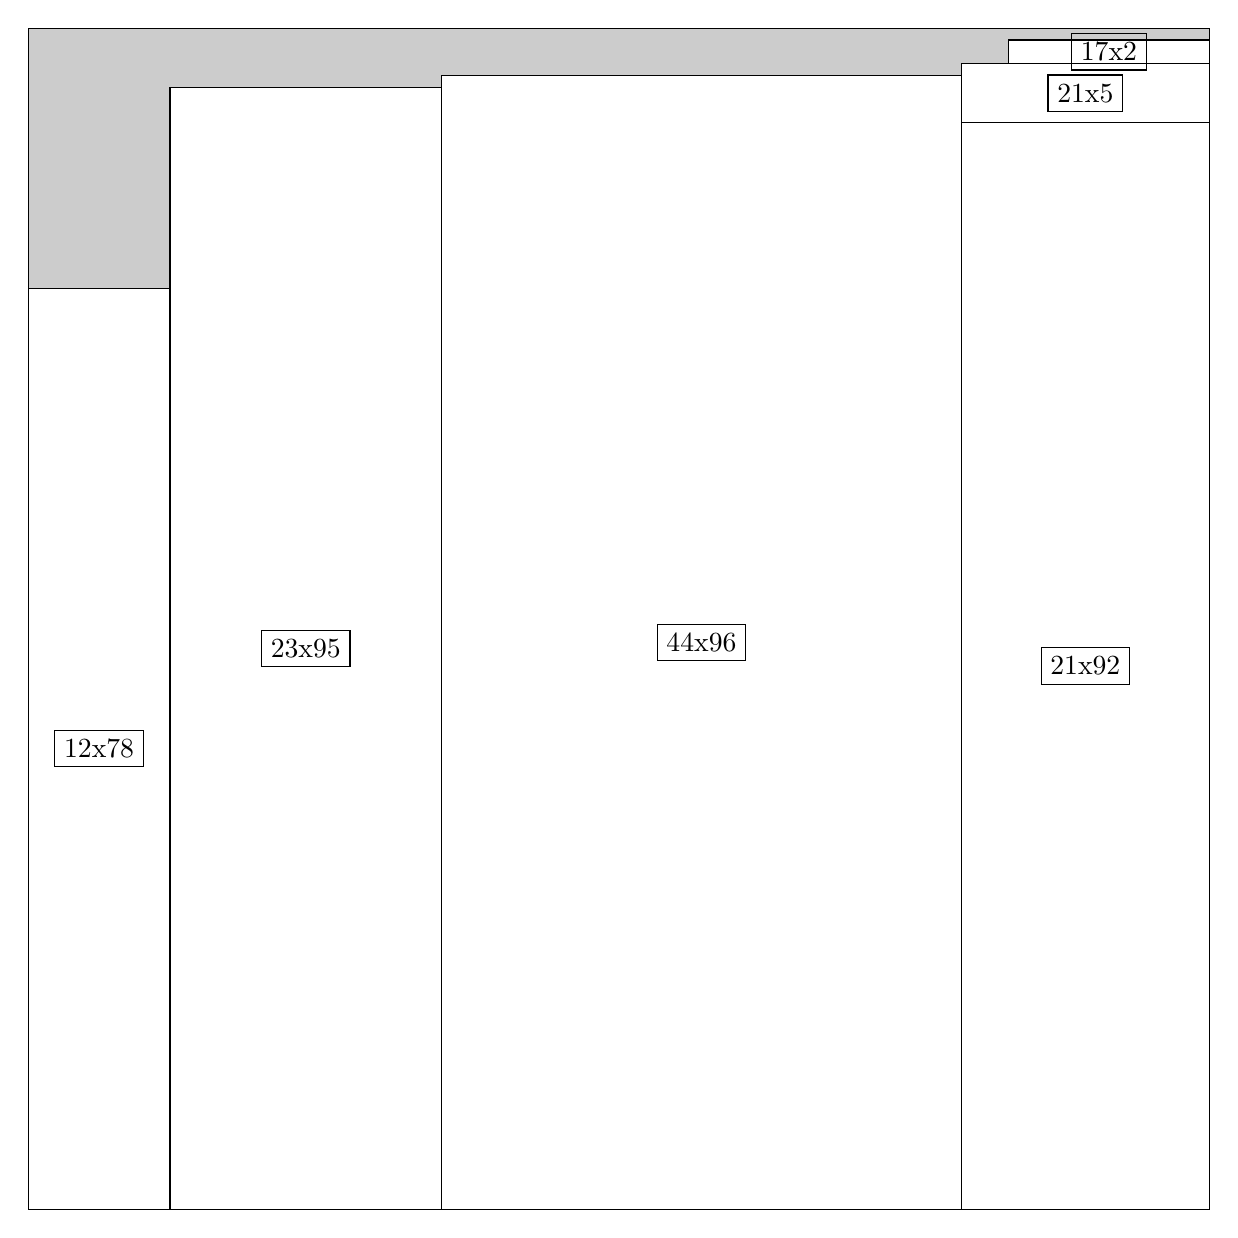
\begin{tikzpicture}[shorten >=1pt,scale=1.0,every node/.style={scale=1.0},->]
\tikzstyle{vertex}=[circle,fill=black!25,minimum size=14pt,inner sep=0pt]
\filldraw[fill=gray!40!white, draw=black] (0,0) rectangle (15.0,15.0);
\foreach \name/\x/\y/\w/\h in {21x92/11.85/0.0/3.15/13.799999999999999,21x5/11.85/13.799999999999999/3.15/0.75,17x2/12.45/14.549999999999999/2.55/0.3,44x96/5.25/0.0/6.6/14.399999999999999,23x95/1.7999999999999998/0.0/3.4499999999999997/14.25,12x78/0.0/0.0/1.7999999999999998/11.7}
\filldraw[fill=white!40!white, draw=black] (\x,\y) rectangle node[draw] (\name) {\name} ++(\w,\h);
\end{tikzpicture}


w =21 , h =92 , x =79 , y =0 , v =1932
\par
w =21 , h =5 , x =79 , y =92 , v =105
\par
w =17 , h =2 , x =83 , y =97 , v =34
\par
w =44 , h =96 , x =35 , y =0 , v =4224
\par
w =23 , h =95 , x =12 , y =0 , v =2185
\par
w =12 , h =78 , x =0 , y =0 , v =936
\par
\newpage


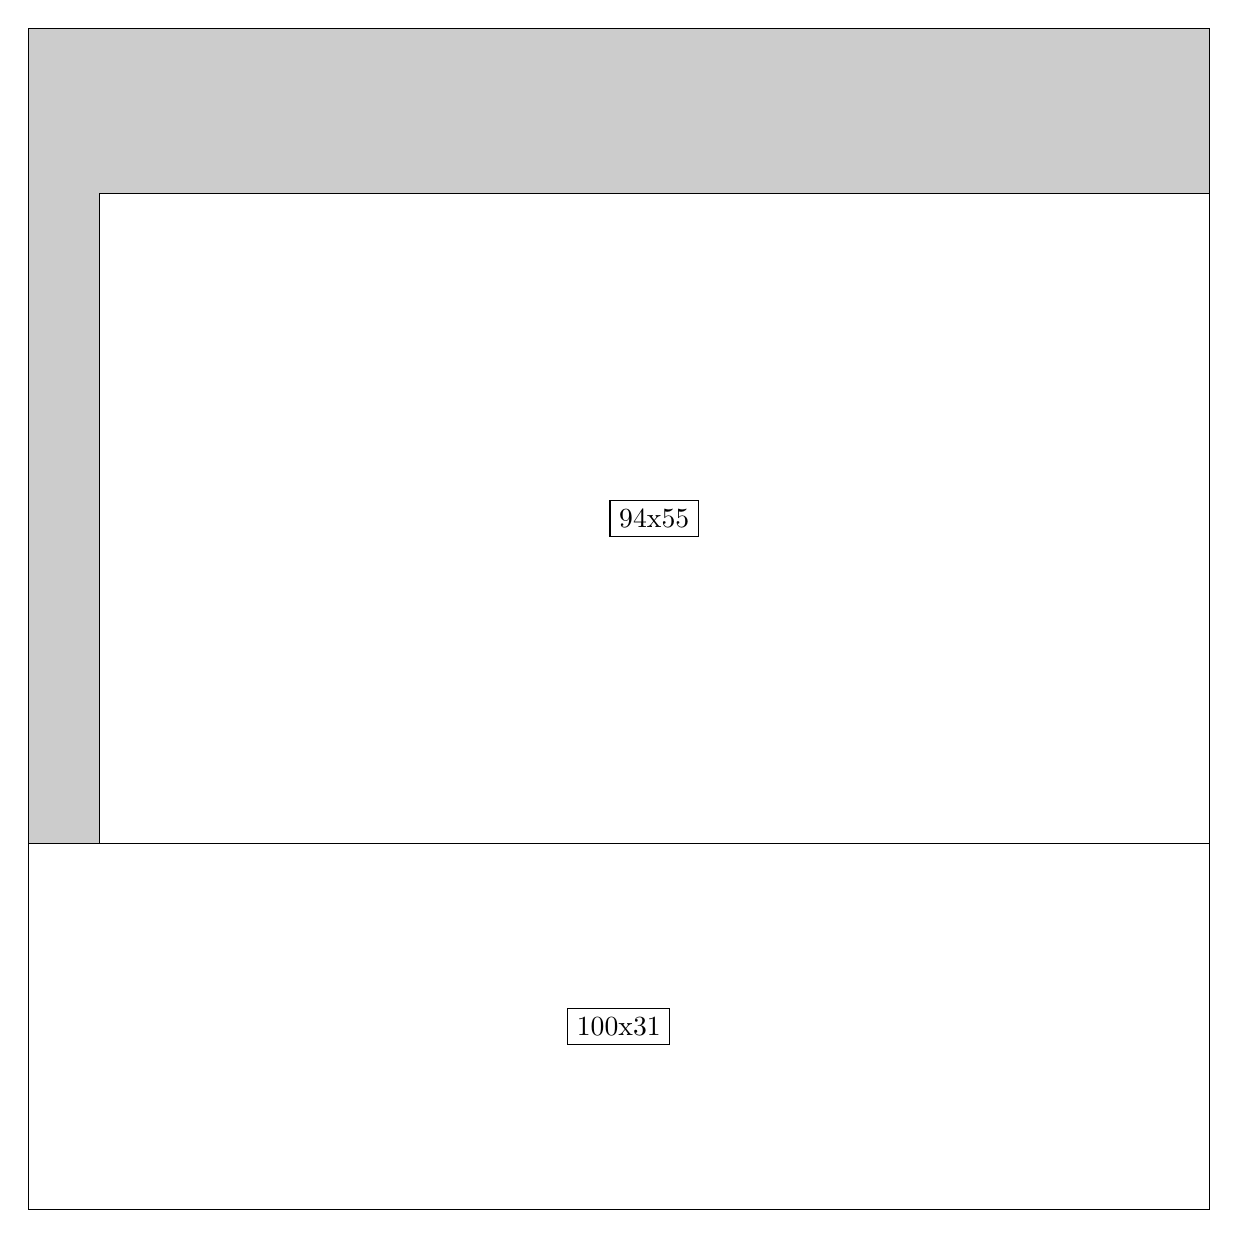
\begin{tikzpicture}[shorten >=1pt,scale=1.0,every node/.style={scale=1.0},->]
\tikzstyle{vertex}=[circle,fill=black!25,minimum size=14pt,inner sep=0pt]
\filldraw[fill=gray!40!white, draw=black] (0,0) rectangle (15.0,15.0);
\foreach \name/\x/\y/\w/\h in {100x31/0.0/0.0/15.0/4.6499999999999995,94x55/0.8999999999999999/4.6499999999999995/14.1/8.25}
\filldraw[fill=white!40!white, draw=black] (\x,\y) rectangle node[draw] (\name) {\name} ++(\w,\h);
\end{tikzpicture}


w =100 , h =31 , x =0 , y =0 , v =3100
\par
w =94 , h =55 , x =6 , y =31 , v =5170
\par
\newpage


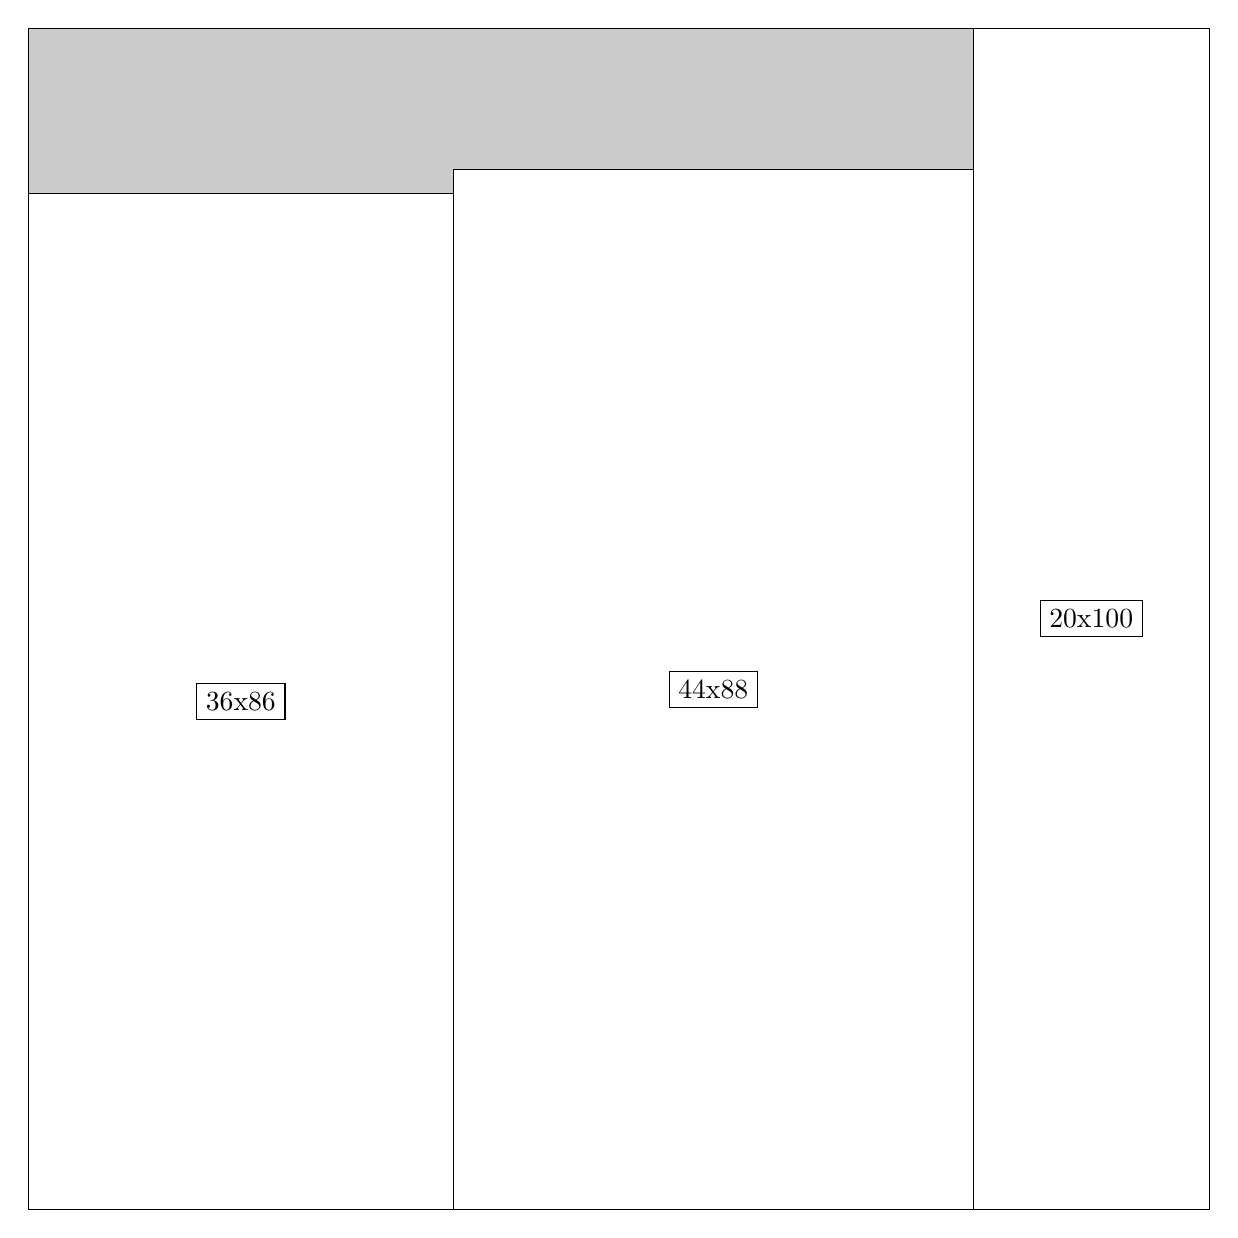
\begin{tikzpicture}[shorten >=1pt,scale=1.0,every node/.style={scale=1.0},->]
\tikzstyle{vertex}=[circle,fill=black!25,minimum size=14pt,inner sep=0pt]
\filldraw[fill=gray!40!white, draw=black] (0,0) rectangle (15.0,15.0);
\foreach \name/\x/\y/\w/\h in {20x100/12.0/0.0/3.0/15.0,44x88/5.3999999999999995/0.0/6.6/13.2,36x86/0.0/0.0/5.3999999999999995/12.9}
\filldraw[fill=white!40!white, draw=black] (\x,\y) rectangle node[draw] (\name) {\name} ++(\w,\h);
\end{tikzpicture}


w =20 , h =100 , x =80 , y =0 , v =2000
\par
w =44 , h =88 , x =36 , y =0 , v =3872
\par
w =36 , h =86 , x =0 , y =0 , v =3096
\par
\newpage


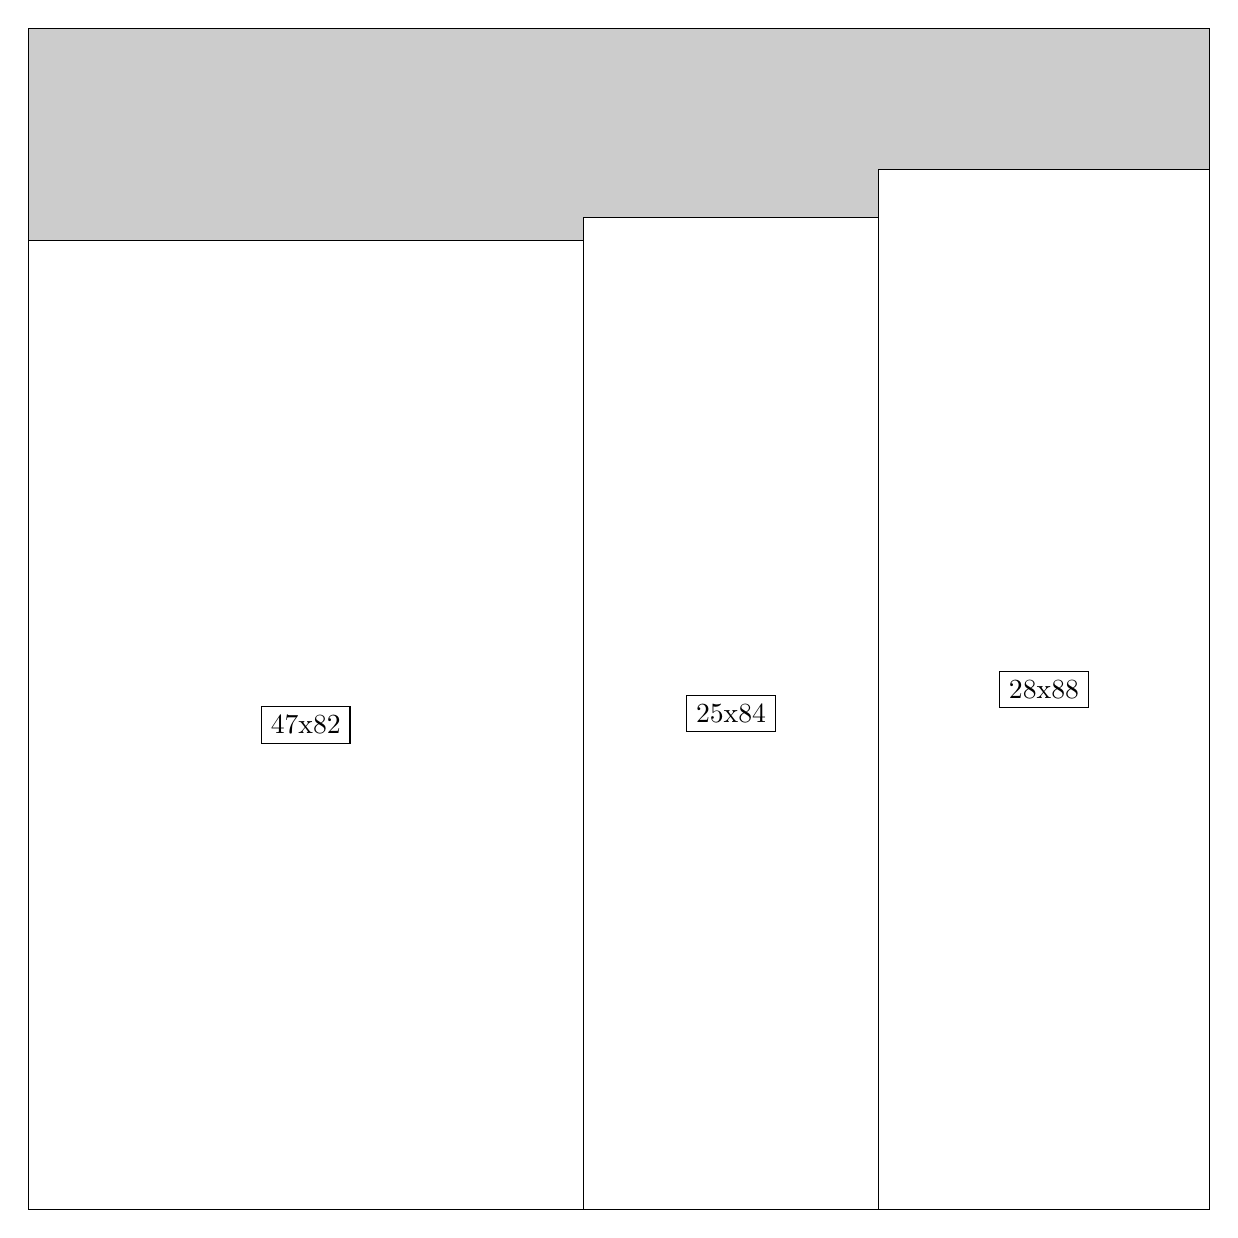
\begin{tikzpicture}[shorten >=1pt,scale=1.0,every node/.style={scale=1.0},->]
\tikzstyle{vertex}=[circle,fill=black!25,minimum size=14pt,inner sep=0pt]
\filldraw[fill=gray!40!white, draw=black] (0,0) rectangle (15.0,15.0);
\foreach \name/\x/\y/\w/\h in {28x88/10.799999999999999/0.0/4.2/13.2,25x84/7.05/0.0/3.75/12.6,47x82/0.0/0.0/7.05/12.299999999999999}
\filldraw[fill=white!40!white, draw=black] (\x,\y) rectangle node[draw] (\name) {\name} ++(\w,\h);
\end{tikzpicture}


w =28 , h =88 , x =72 , y =0 , v =2464
\par
w =25 , h =84 , x =47 , y =0 , v =2100
\par
w =47 , h =82 , x =0 , y =0 , v =3854
\par
\newpage


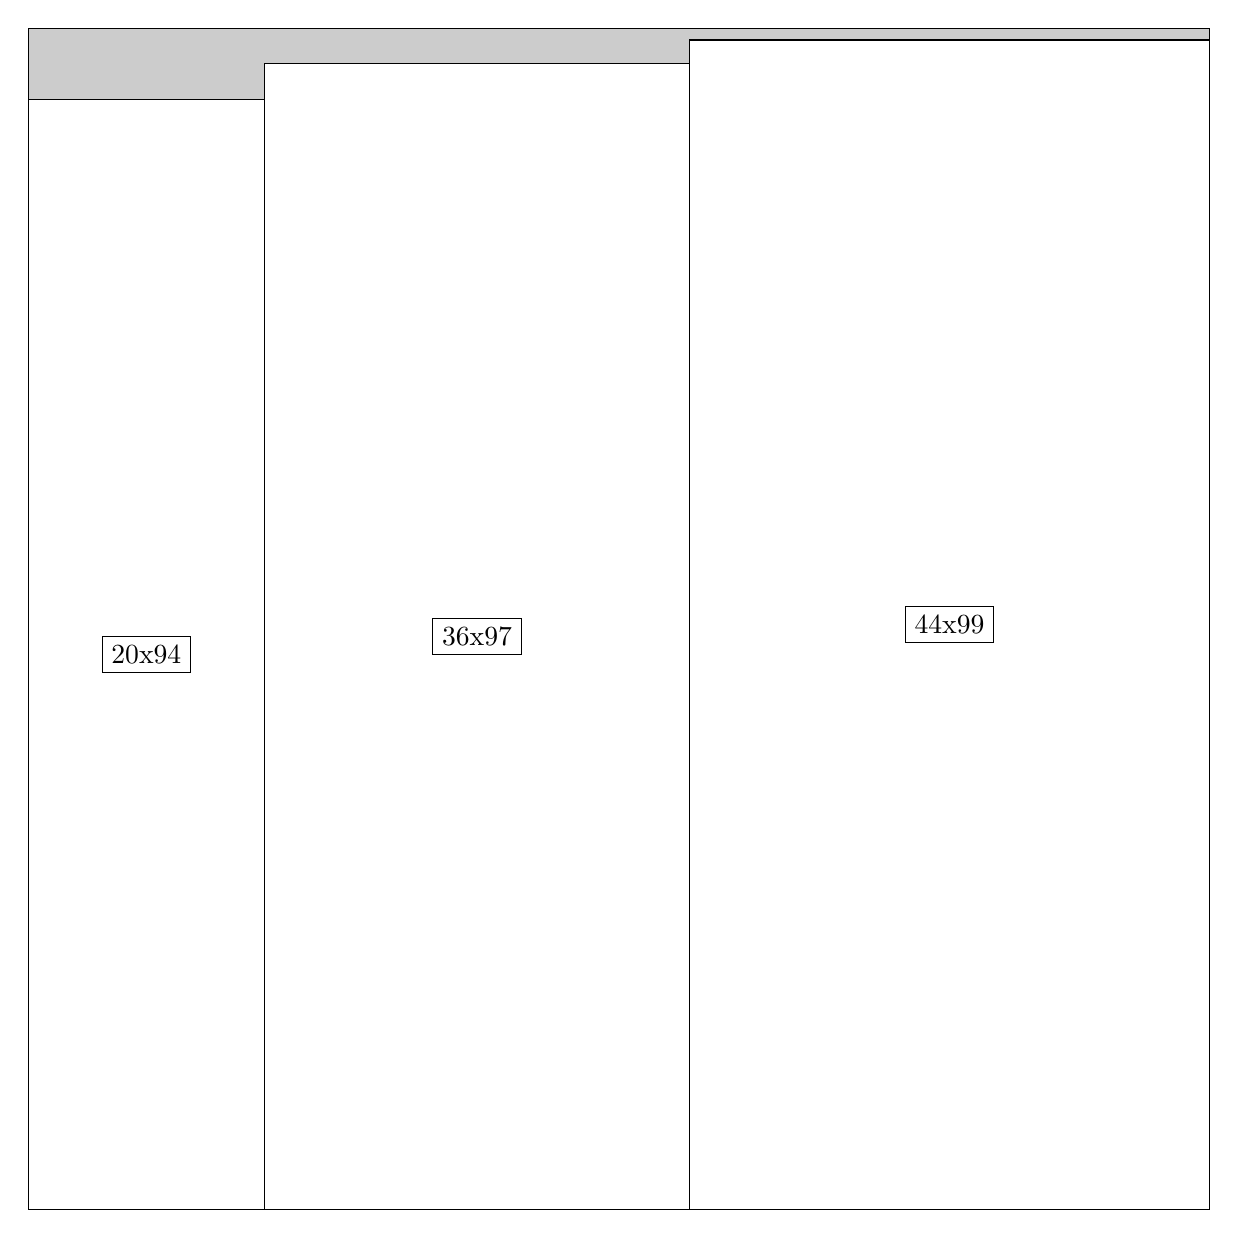
\begin{tikzpicture}[shorten >=1pt,scale=1.0,every node/.style={scale=1.0},->]
\tikzstyle{vertex}=[circle,fill=black!25,minimum size=14pt,inner sep=0pt]
\filldraw[fill=gray!40!white, draw=black] (0,0) rectangle (15.0,15.0);
\foreach \name/\x/\y/\w/\h in {44x99/8.4/0.0/6.6/14.85,36x97/3.0/0.0/5.3999999999999995/14.549999999999999,20x94/0.0/0.0/3.0/14.1}
\filldraw[fill=white!40!white, draw=black] (\x,\y) rectangle node[draw] (\name) {\name} ++(\w,\h);
\end{tikzpicture}


w =44 , h =99 , x =56 , y =0 , v =4356
\par
w =36 , h =97 , x =20 , y =0 , v =3492
\par
w =20 , h =94 , x =0 , y =0 , v =1880
\par
\newpage


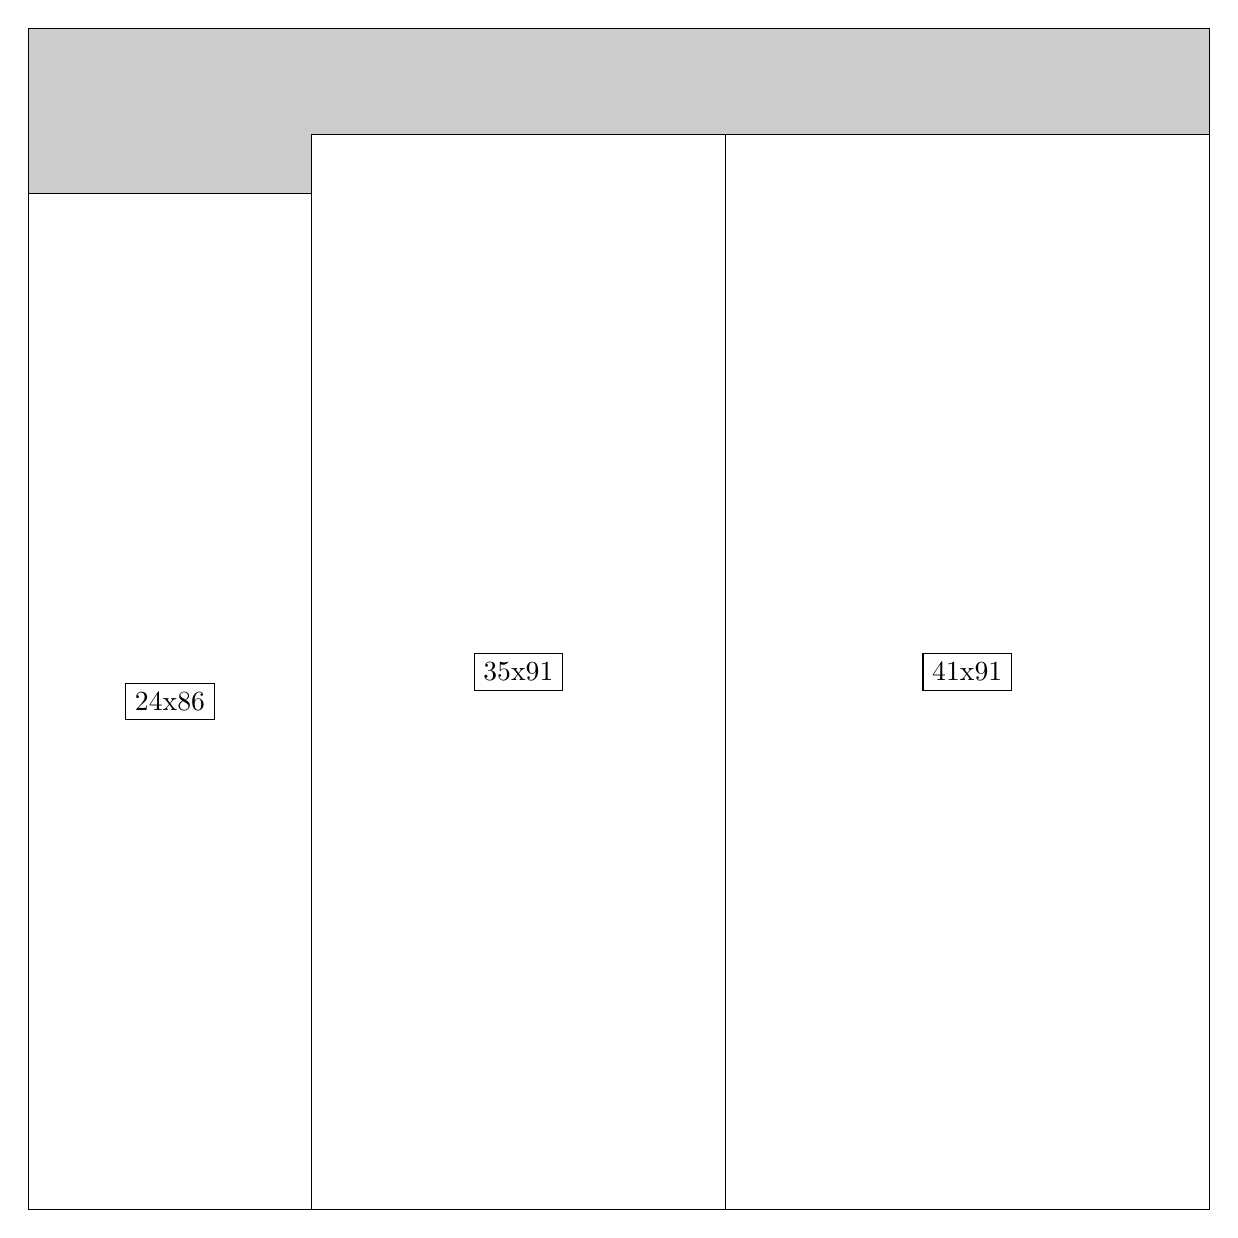
\begin{tikzpicture}[shorten >=1pt,scale=1.0,every node/.style={scale=1.0},->]
\tikzstyle{vertex}=[circle,fill=black!25,minimum size=14pt,inner sep=0pt]
\filldraw[fill=gray!40!white, draw=black] (0,0) rectangle (15.0,15.0);
\foreach \name/\x/\y/\w/\h in {41x91/8.85/0.0/6.1499999999999995/13.65,35x91/3.5999999999999996/0.0/5.25/13.65,24x86/0.0/0.0/3.5999999999999996/12.9}
\filldraw[fill=white!40!white, draw=black] (\x,\y) rectangle node[draw] (\name) {\name} ++(\w,\h);
\end{tikzpicture}


w =41 , h =91 , x =59 , y =0 , v =3731
\par
w =35 , h =91 , x =24 , y =0 , v =3185
\par
w =24 , h =86 , x =0 , y =0 , v =2064
\par
\newpage


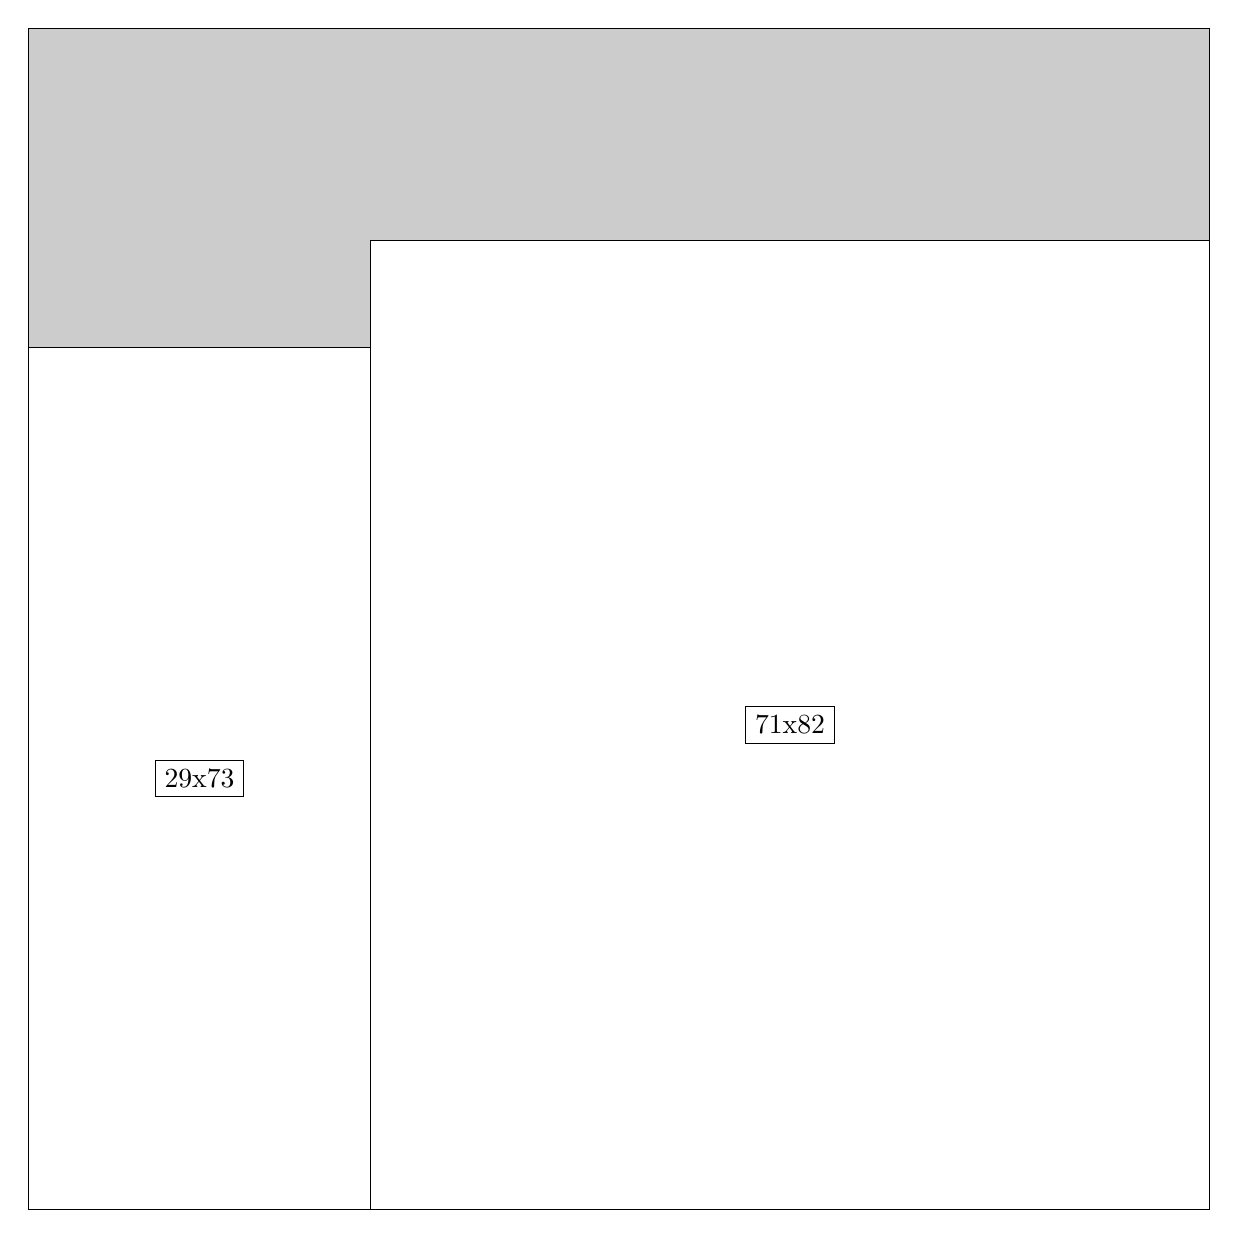
\begin{tikzpicture}[shorten >=1pt,scale=1.0,every node/.style={scale=1.0},->]
\tikzstyle{vertex}=[circle,fill=black!25,minimum size=14pt,inner sep=0pt]
\filldraw[fill=gray!40!white, draw=black] (0,0) rectangle (15.0,15.0);
\foreach \name/\x/\y/\w/\h in {71x82/4.35/0.0/10.65/12.299999999999999,29x73/0.0/0.0/4.35/10.95}
\filldraw[fill=white!40!white, draw=black] (\x,\y) rectangle node[draw] (\name) {\name} ++(\w,\h);
\end{tikzpicture}


w =71 , h =82 , x =29 , y =0 , v =5822
\par
w =29 , h =73 , x =0 , y =0 , v =2117
\par
\newpage


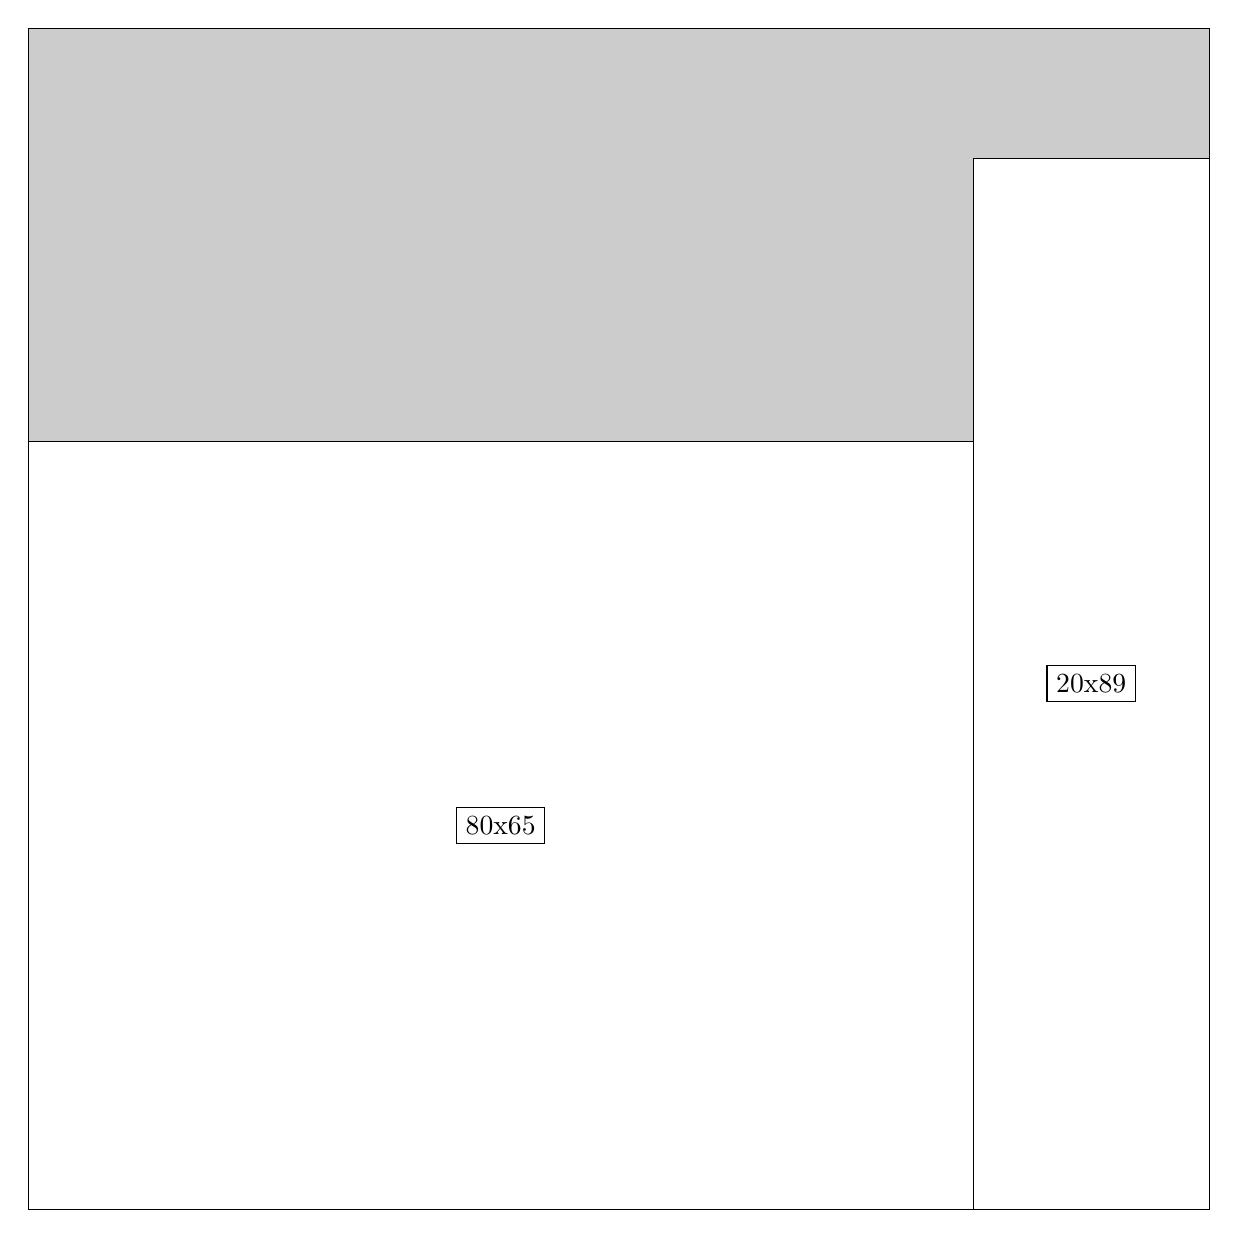
\begin{tikzpicture}[shorten >=1pt,scale=1.0,every node/.style={scale=1.0},->]
\tikzstyle{vertex}=[circle,fill=black!25,minimum size=14pt,inner sep=0pt]
\filldraw[fill=gray!40!white, draw=black] (0,0) rectangle (15.0,15.0);
\foreach \name/\x/\y/\w/\h in {20x89/12.0/0.0/3.0/13.35,80x65/0.0/0.0/12.0/9.75}
\filldraw[fill=white!40!white, draw=black] (\x,\y) rectangle node[draw] (\name) {\name} ++(\w,\h);
\end{tikzpicture}


w =20 , h =89 , x =80 , y =0 , v =1780
\par
w =80 , h =65 , x =0 , y =0 , v =5200
\par
\newpage


\end{document}